% Generado desde docs/INFORME.md. Editar libremente.

\section{10. Backend completo e integración verificable}

\subsection{Qué se entrega}

{\small
\setlength{\tabcolsep}{3pt}\renewcommand{\arraystretch}{1.15}
\begin{longtable}{|>{\raggedright\arraybackslash}p{\dimexpr 0.3248\linewidth-2\tabcolsep\relax}|>{\raggedright\arraybackslash}p{\dimexpr 0.6752\linewidth-2\tabcolsep\relax}|}
\hline
\textbf{Pieza} & \textbf{Dónde} \\ \hline
\endfirsthead
\hline
\textbf{Pieza} & \textbf{Dónde} \\ \hline
\endhead
Código del frontend & \texttt{frontend/\allowbreak{}} \\ \hline
Código del backend & \texttt{gateway/\allowbreak{}}, \texttt{auth-\allowbreak{}service/\allowbreak{}}, \texttt{graphql-\allowbreak{}gateway/\allowbreak{}}, \texttt{servicios/\allowbreak{}} \\ \hline
Despliegue reproducible & \texttt{docker-\allowbreak{}compose.\allowbreak{}yml}, \texttt{Dockerfile} de cada componente, \texttt{vault/\allowbreak{}} \\ \hline
Persistencia y creación & MongoDB con una base y un usuario por servicio; índices creados al arrancar (\texttt{preparar} en cada servicio); datos ficticios con \texttt{servicios/\allowbreak{}scripts/\allowbreak{}semilla.\allowbreak{}py} \\ \hline
Contratos REST & Sección 1 y OpenAPI de cada servicio \\ \hline
Contrato GraphQL & Sección 8 y \texttt{graphql-\allowbreak{}gateway/\allowbreak{}src/\allowbreak{}graphql/\allowbreak{}esquema.\allowbreak{}js} \\ \hline
Contratos gRPC & No aplica (ADR 0001) \\ \hline
Pruebas automatizadas & 86 unitarias y de integración + 23 de punta a punta (contra Docker, con TLS) + recorrido de pantallas + carga \\ \hline
Instrucciones & \texttt{README.\allowbreak{}md} \\ \hline
\end{longtable}
}

\subsection{Pruebas y resultados}

{\small
\setlength{\tabcolsep}{3pt}\renewcommand{\arraystretch}{1.15}
\begin{longtable}{|>{\raggedright\arraybackslash}p{\dimexpr 0.2074\linewidth-2\tabcolsep\relax}|>{\raggedleft\arraybackslash}p{\dimexpr 0.2069\linewidth-2\tabcolsep\relax}|>{\raggedright\arraybackslash}p{\dimexpr 0.4017\linewidth-2\tabcolsep\relax}|>{\raggedright\arraybackslash}p{\dimexpr 0.1840\linewidth-2\tabcolsep\relax}|}
\hline
\textbf{Conjunto} & \textbf{Cantidad} & \textbf{Qué cubre} & \textbf{Resultado} \\ \hline
\endfirsthead
\hline
\textbf{Conjunto} & \textbf{Cantidad} & \textbf{Qué cubre} & \textbf{Resultado} \\ \hline
\endhead
\texttt{servicios/\allowbreak{}tests} (pytest) & 37 & Reglas de cada servicio, propiedad, cotización, stock, idempotencia, firma, Vault caído (503), servicio caído (502), datos de ejemplo, URI de Mongo con TLS & 37/37 \\ \hline
\texttt{auth-\allowbreak{}service/\allowbreak{}test} & 20 & Login, bloqueo, expiración, revocación, verificación, permisos por cliente, hash y pepper, Vault sellado & 20/20 \\ \hline
\texttt{gateway/\allowbreak{}test} & 18 & Matriz de rutas, roles, cabeceras falsificadas, cookie, CSRF, webhook, Vault y servicio caídos, límite, healthcheck, HSTS & 18/18 \\ \hline
\texttt{graphql-\allowbreak{}gateway/\allowbreak{}test} & 11 & Agregación, batching, identidad, autorización por campo, error parcial, límites, paginación & 11/11 \\ \hline
\texttt{pruebas/\allowbreak{}e2e/\allowbreak{}casos.\allowbreak{}py -\allowbreak{}-\allowbreak{}docker} & 23 & Casos del módulo 7 y del 10 contra el sistema levantado en Docker, por HTTPS; los casos 7.9, 7.10 y 10.7 se ejecutan dentro de la red privada & 23/23 \\ \hline
\texttt{pruebas/\allowbreak{}e2e/\allowbreak{}pantallas.\allowbreak{}py} & 16 pantallas de escritorio + 6 móviles & Flujos principales en el navegador, en escritorio (1280×900) y en móvil (375×812, táctil) & Completo, sin errores de consola \\ \hline
\texttt{pruebas/\allowbreak{}carga/\allowbreak{}carga.\allowbreak{}mjs} & 3 escenarios & Rendimiento contra el sistema en Docker & 0 \% de error \\ \hline
\end{longtable}
}

\subsection{Evidencia en móvil}

El recorrido repite seis pantallas en un teléfono emulado (375×812, táctil), contra el mismo sistema en Docker y las mismas APIs: inicio, menú, checkout, seguimiento del pedido, mis pedidos y despacho (\texttt{pantallas/\allowbreak{}m01-\allowbreak{}inicio-\allowbreak{}movil.\allowbreak{}png} a \texttt{m06-\allowbreak{}despacho-\allowbreak{}movil.\allowbreak{}png}). Para cada una el script comprueba que no hay scroll horizontal (\texttt{desbordeHorizontalMovil} en \texttt{pantallas/\allowbreak{}recorrido.\allowbreak{}json}: las seis en \texttt{false}). Los flujos de cocina y administración se verificaron solo en escritorio; el resto de los flujos se comparten entre ambos tamaños, porque es la misma SPA con diseño responsivo.


Además, \texttt{pruebas/\allowbreak{}e2e/\allowbreak{}movil.\allowbreak{}py} recorre en móvil (390×812, táctil, escala 2) una compra completa por HTTPS: inicio, menú, ingreso, checkout, pago, pasarela, pedido pagado con boleta e historial (\texttt{evidencias/\allowbreak{}movil/\allowbreak{}01-\allowbreak{}inicio.\allowbreak{}png} a \texttt{08-\allowbreak{}mis-\allowbreak{}pedidos.\allowbreak{}png}). Comprueba que todas las pantallas se sirven por HTTPS y que ninguna tiene scroll horizontal (\texttt{evidencias/\allowbreak{}movil/\allowbreak{}recorrido.\allowbreak{}json}), con 0 errores de consola. Es emulación de teléfono en Chromium, no un dispositivo real.


\subsection{Evidencia en navegador real}

\texttt{evidencias/\allowbreak{}navegador-\allowbreak{}real/\allowbreak{}} tiene 8 capturas de una compra completa hecha en Microsoft Edge por HTTPS (pedido PF-00086, pago aprobado en la pasarela de \texttt{https:\allowbreak{}/\allowbreak{}/\allowbreak{}localhost:\allowbreak{}9000}, boleta N° 83) y \texttt{datos-\allowbreak{}navegador.\allowbreak{}json} con el navegador, el protocolo, las URLs visitadas y la cabecera HSTS. Las capturas muestran la página y no la barra de direcciones; el protocolo consta en ese archivo. Antes de capturar se aceptó a mano la advertencia que el antivirus muestra por el certificado de prueba.


\subsection{Capturas de la ejecución}

Todas salen del sistema levantado en Docker, por HTTPS, con datos ficticios. Las de escritorio y las del teléfono emulado las generan \texttt{pruebas/\allowbreak{}e2e/\allowbreak{}pantallas.\allowbreak{}py} y \texttt{pruebas/\allowbreak{}e2e/\allowbreak{}movil.\allowbreak{}py}; las del navegador real se tomaron a mano en Edge. Las tres capturas de la sección 8 (pedido con pagos, vista del administrador y reportes) no se repiten aquí.


\subsubsection{Escritorio (Chromium, 1280×900): compra, cocina, despacho y administración}

\begin{figure}[H]\centering
\begin{minipage}[t]{0.485\linewidth}\centering
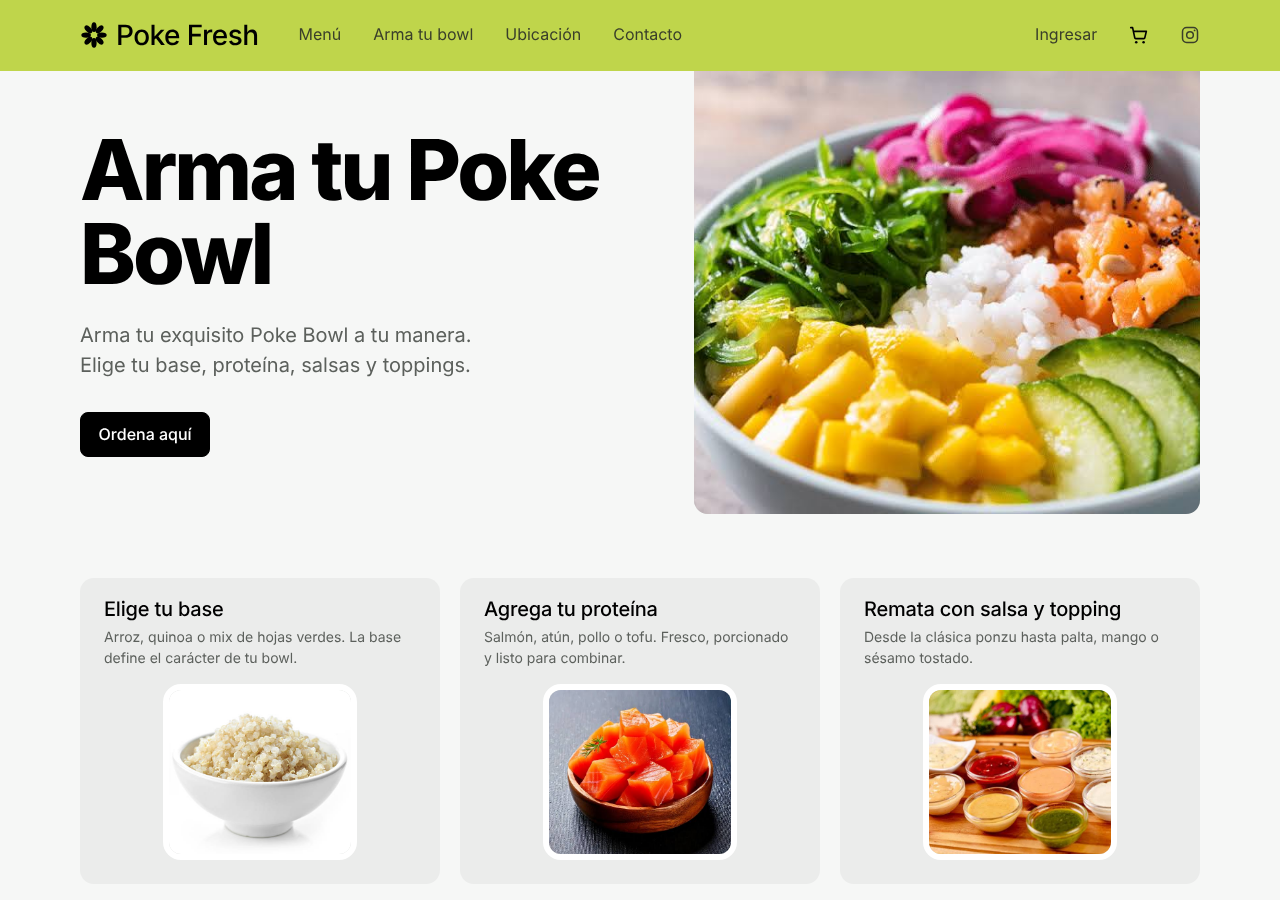
\includegraphics[width=\linewidth,height=0.42\textheight,keepaspectratio]{../evidencias/pantallas/01-inicio.png}
\captionof{figure}{Inicio: la tienda pública}
\end{minipage}\hfill
\begin{minipage}[t]{0.485\linewidth}\centering
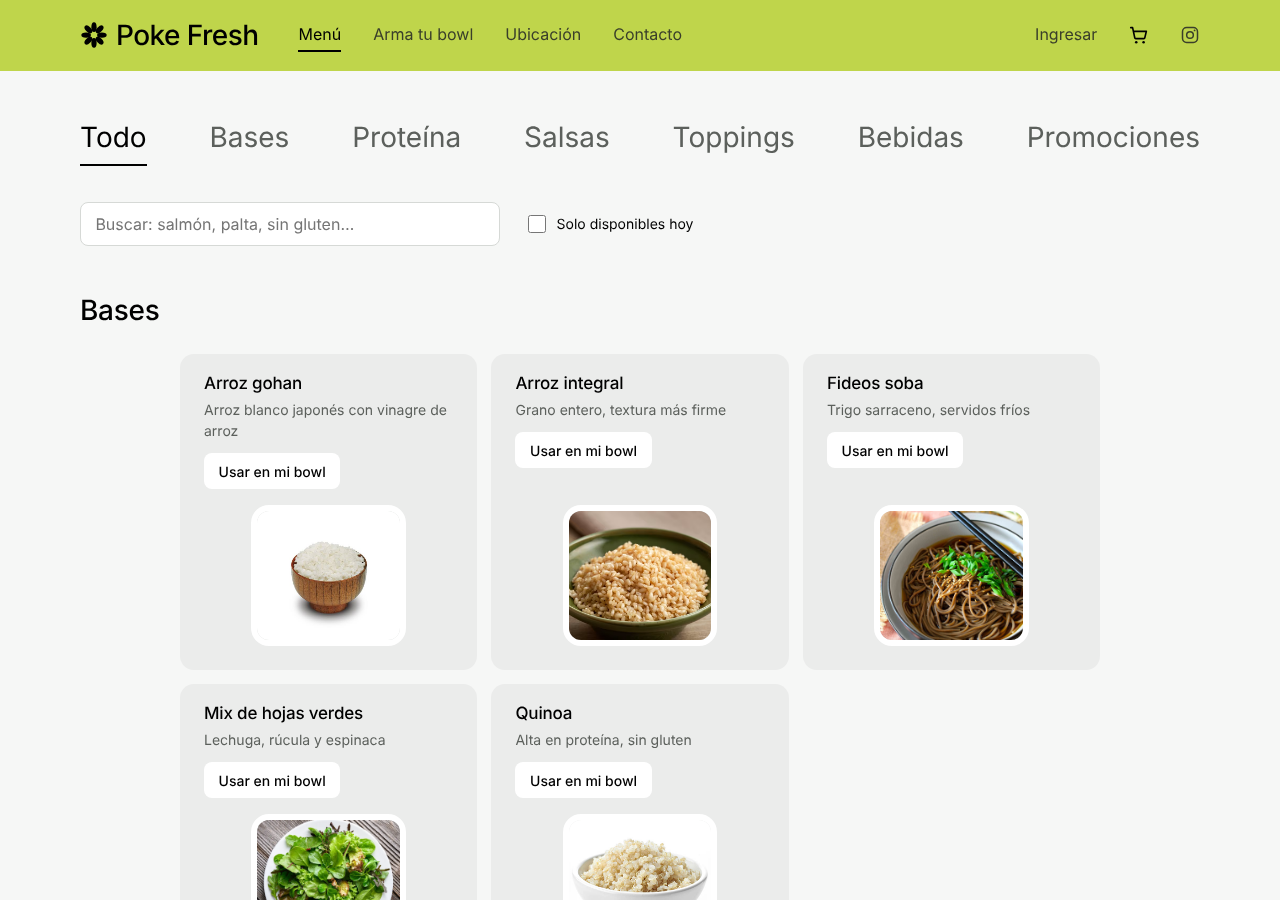
\includegraphics[width=\linewidth,height=0.42\textheight,keepaspectratio]{../evidencias/pantallas/02-menu-desde-inventario.png}
\captionof{figure}{Menú cargado desde el servicio de inventario}
\end{minipage}
\end{figure}

\begin{figure}[H]\centering
\begin{minipage}[t]{0.485\linewidth}\centering
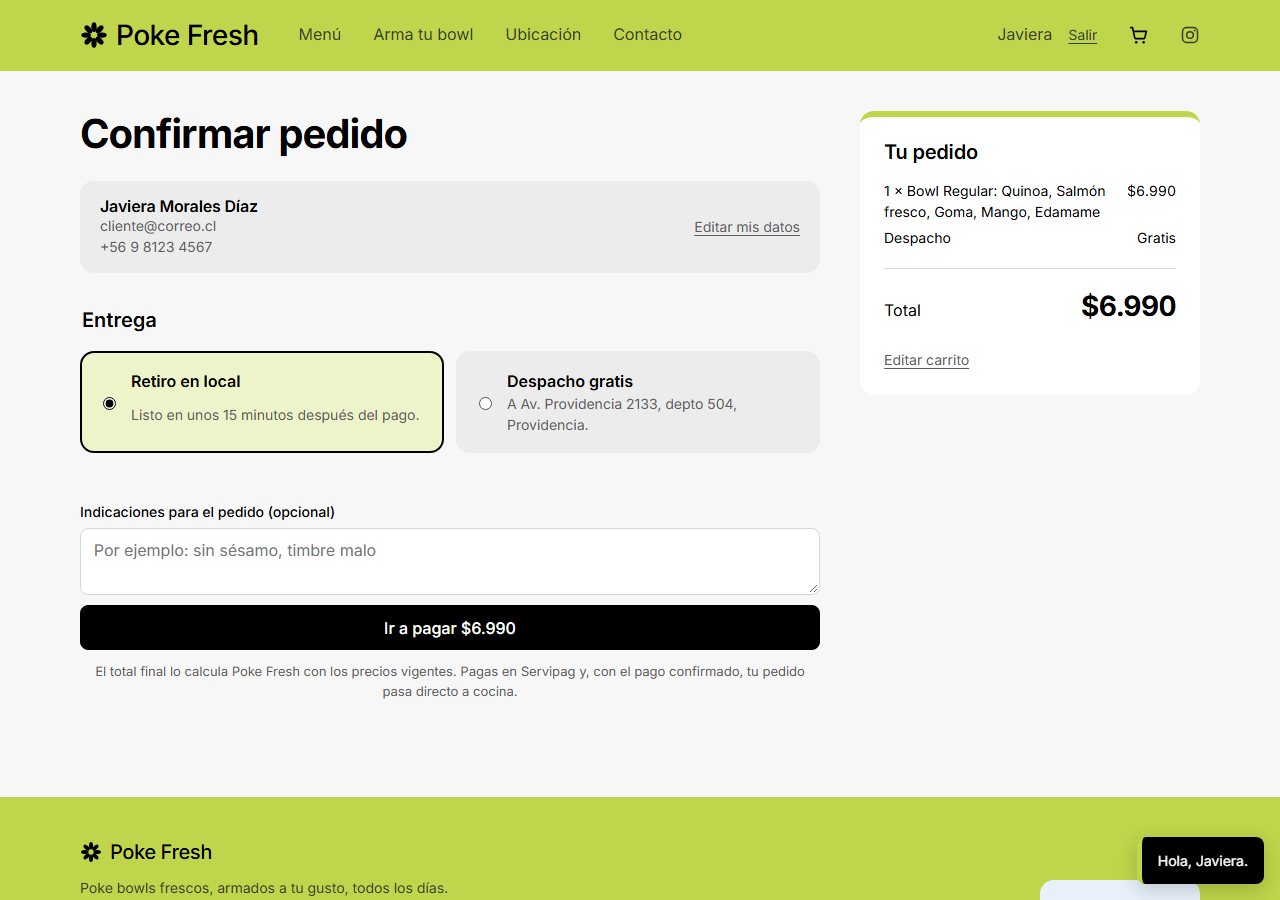
\includegraphics[width=\linewidth,height=0.42\textheight,keepaspectratio]{../evidencias/pantallas/03-checkout.png}
\captionof{figure}{Confirmar pedido: solo se manda la selección}
\end{minipage}\hfill
\begin{minipage}[t]{0.485\linewidth}\centering
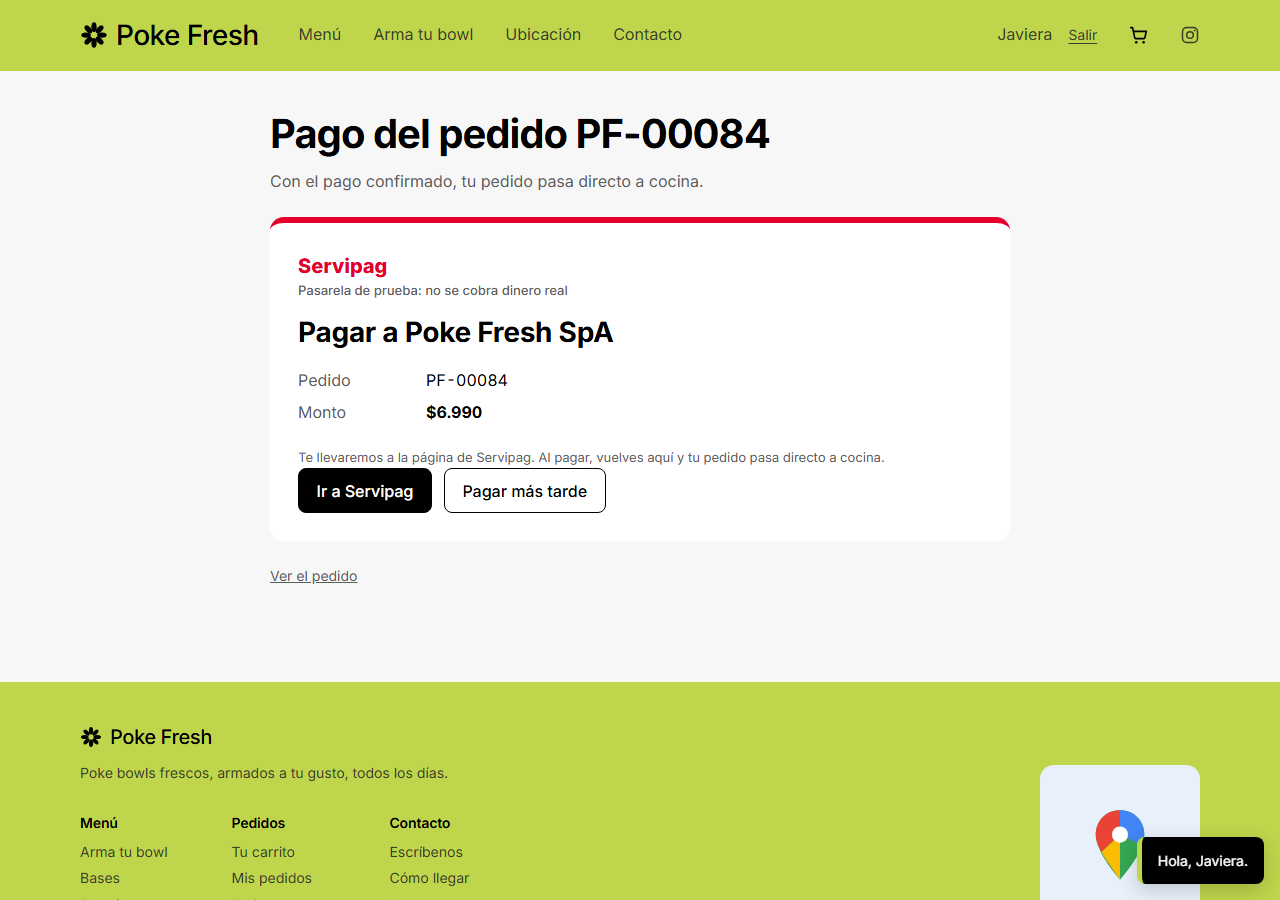
\includegraphics[width=\linewidth,height=0.42\textheight,keepaspectratio]{../evidencias/pantallas/04-pago.png}
\captionof{figure}{Pago: el pedido queda pendiente hasta que la pasarela confirme}
\end{minipage}
\end{figure}

\begin{figure}[H]
\centering
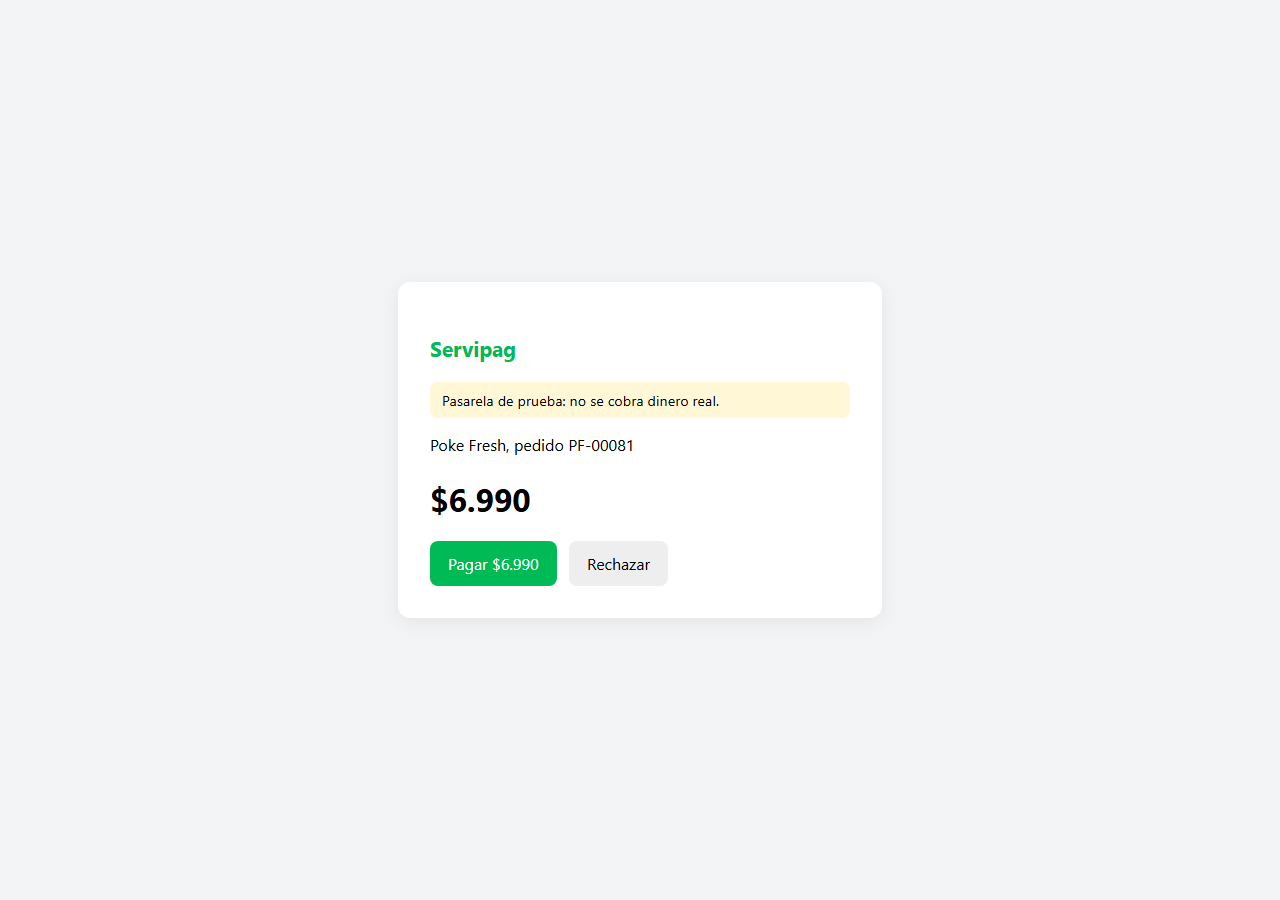
\includegraphics[width=\linewidth,height=0.85\textheight,keepaspectratio]{../evidencias/pantallas/05-pasarela-servipag.png}
\caption{Pasarela de pago simulada (Servipag), en el puerto 9000}
\end{figure}

\begin{figure}[H]\centering
\begin{minipage}[t]{0.485\linewidth}\centering
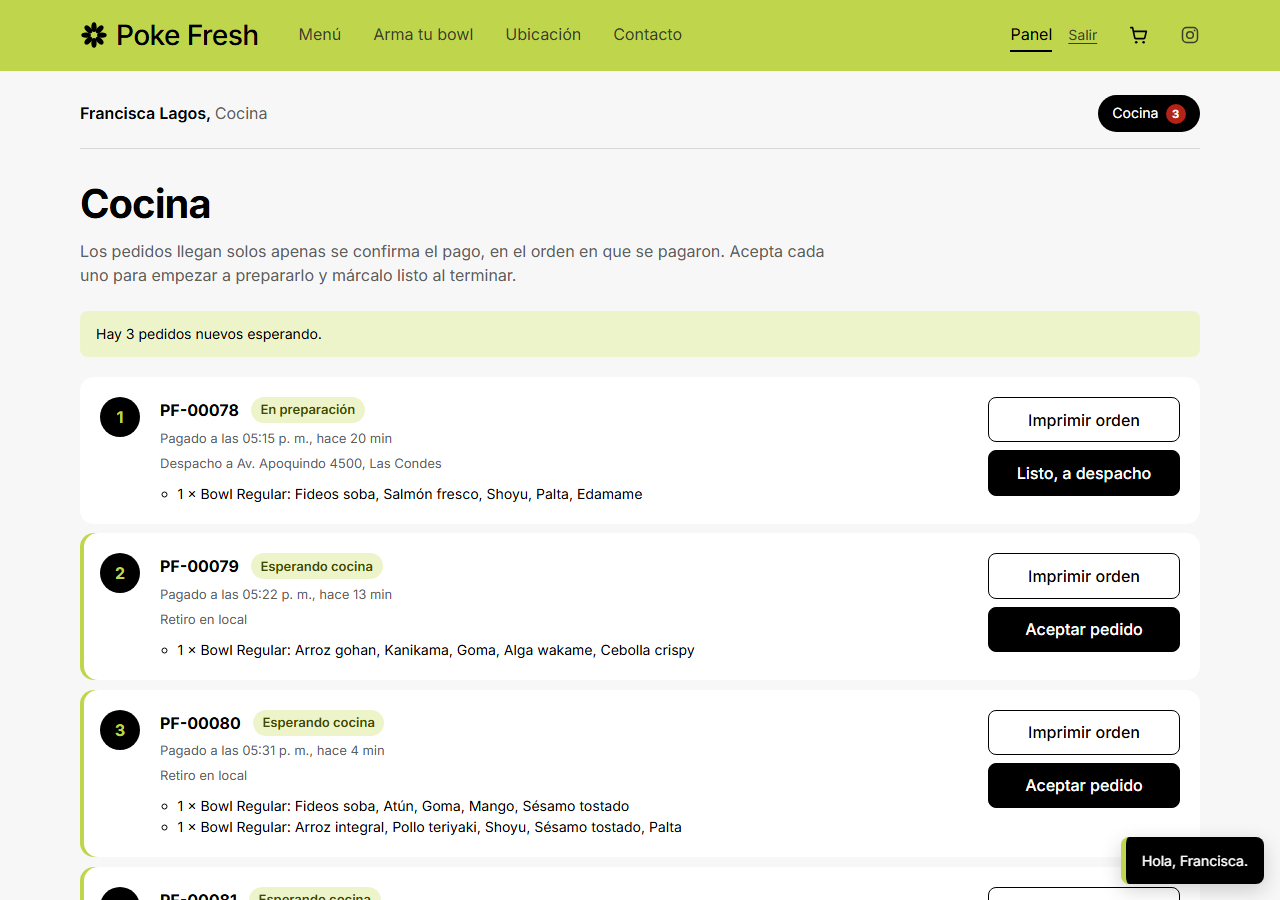
\includegraphics[width=\linewidth,height=0.42\textheight,keepaspectratio]{../evidencias/pantallas/07-cocina.png}
\captionof{figure}{Cocina: cola de pedidos pagados, en orden de llegada}
\end{minipage}\hfill
\begin{minipage}[t]{0.485\linewidth}\centering
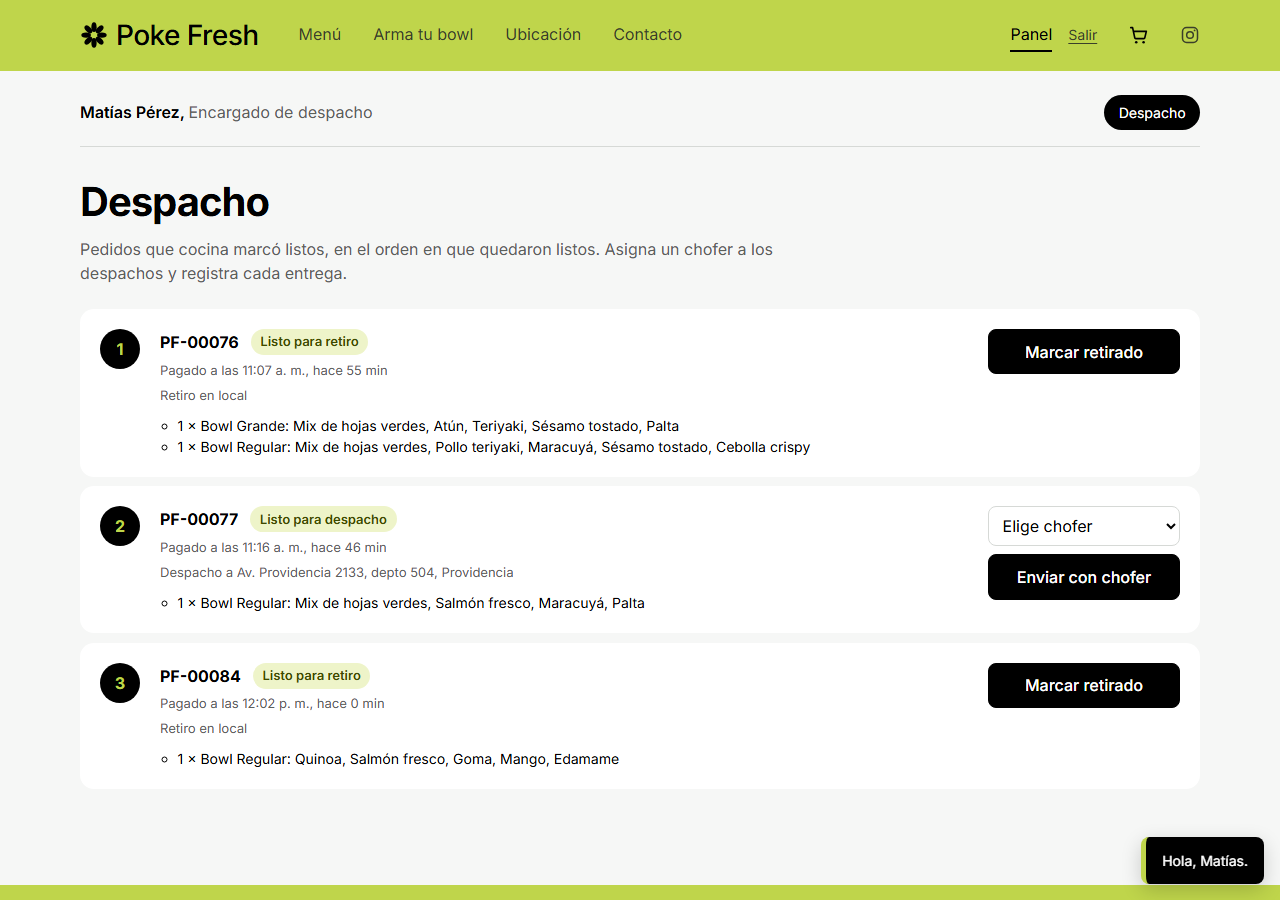
\includegraphics[width=\linewidth,height=0.42\textheight,keepaspectratio]{../evidencias/pantallas/08-despacho.png}
\captionof{figure}{Despacho: pedidos listos para entregar}
\end{minipage}
\end{figure}

\begin{figure}[H]
\centering
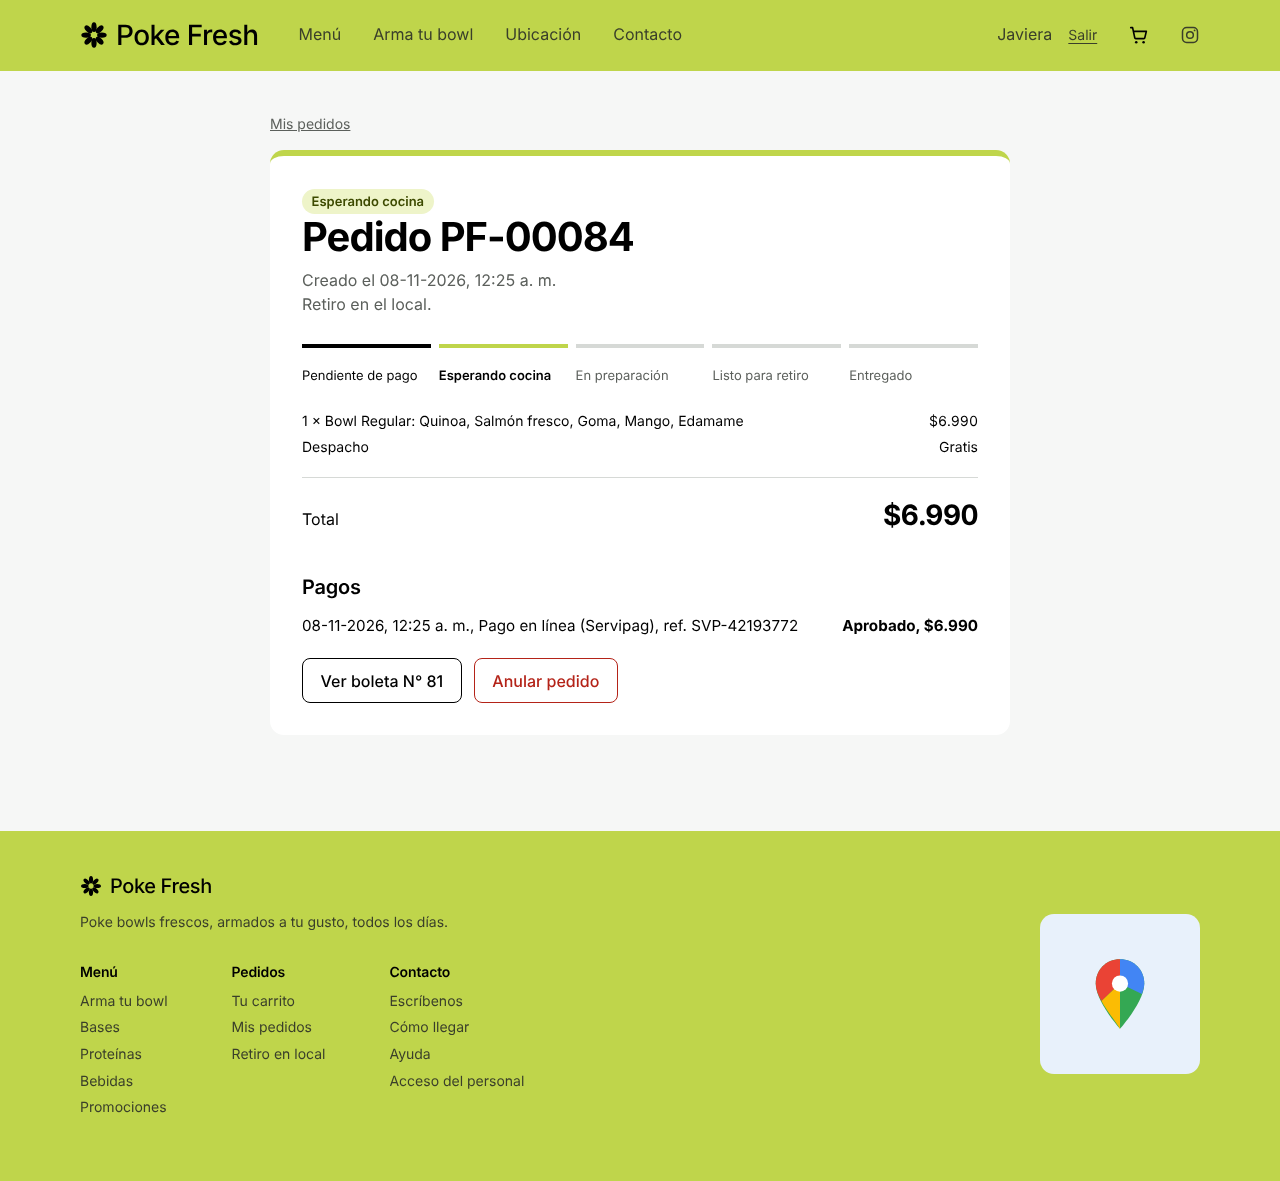
\includegraphics[width=\linewidth,height=0.85\textheight,keepaspectratio]{../evidencias/pantallas/09-seguimiento-entregado.png}
\caption{Seguimiento: el pedido en estado Entregado, con su boleta}
\end{figure}

\begin{figure}[H]
\centering
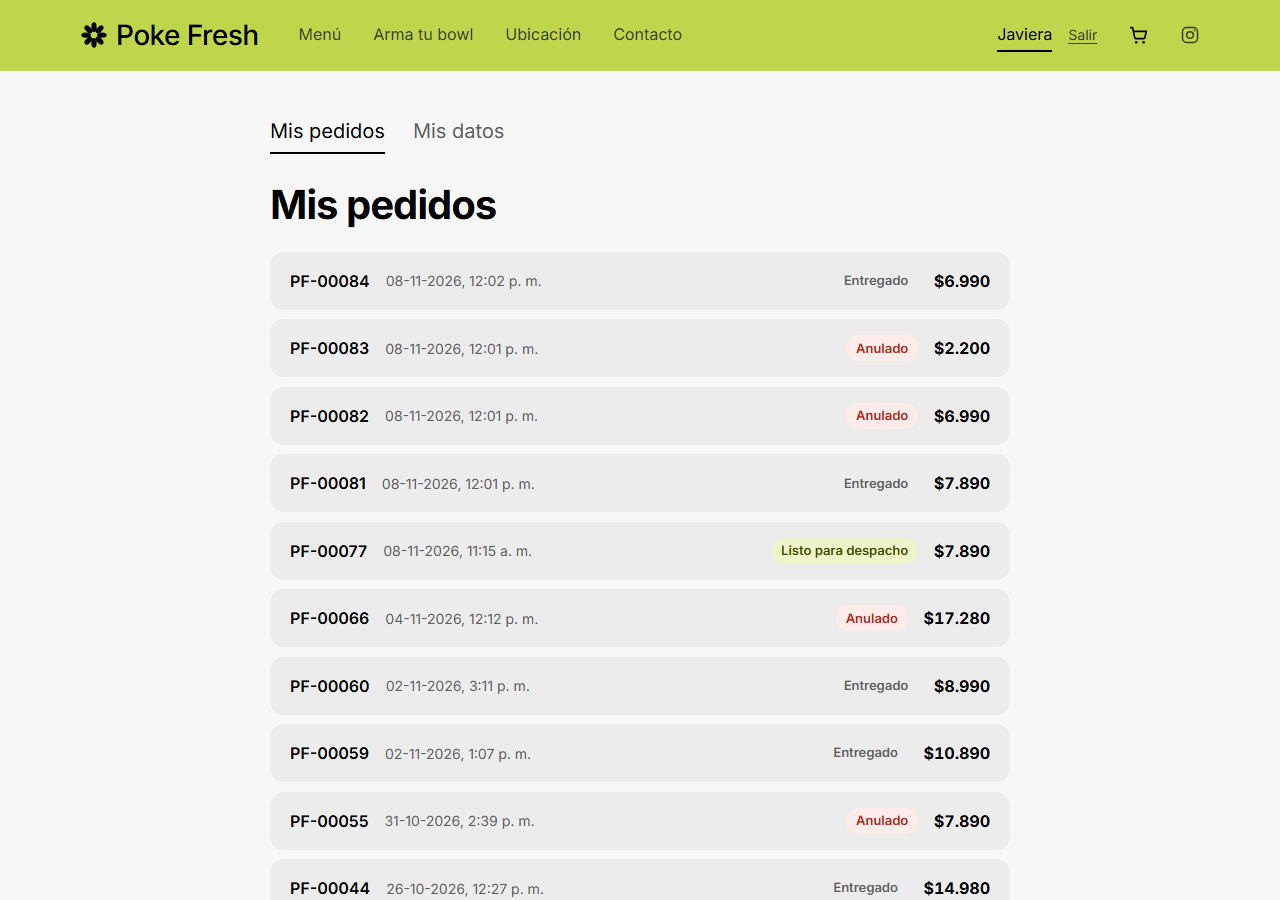
\includegraphics[width=\linewidth,height=0.85\textheight,keepaspectratio]{../evidencias/pantallas/10-mis-pedidos.png}
\caption{Mis pedidos: historial del cliente}
\end{figure}

\begin{figure}[H]\centering
\begin{minipage}[t]{0.485\linewidth}\centering
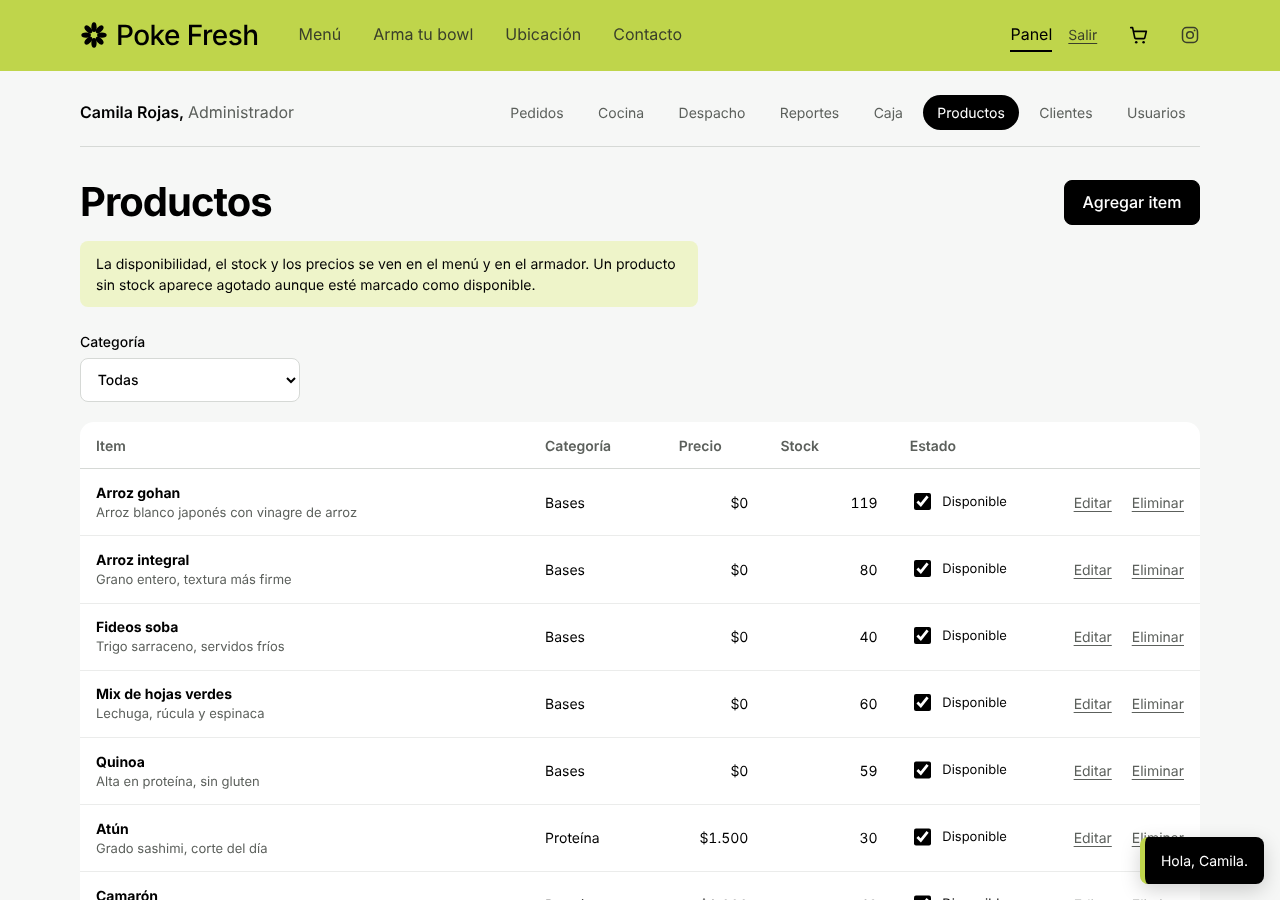
\includegraphics[width=\linewidth,height=0.42\textheight,keepaspectratio]{../evidencias/pantallas/12-productos-stock.png}
\captionof{figure}{Administración: productos y stock}
\end{minipage}\hfill
\begin{minipage}[t]{0.485\linewidth}\centering
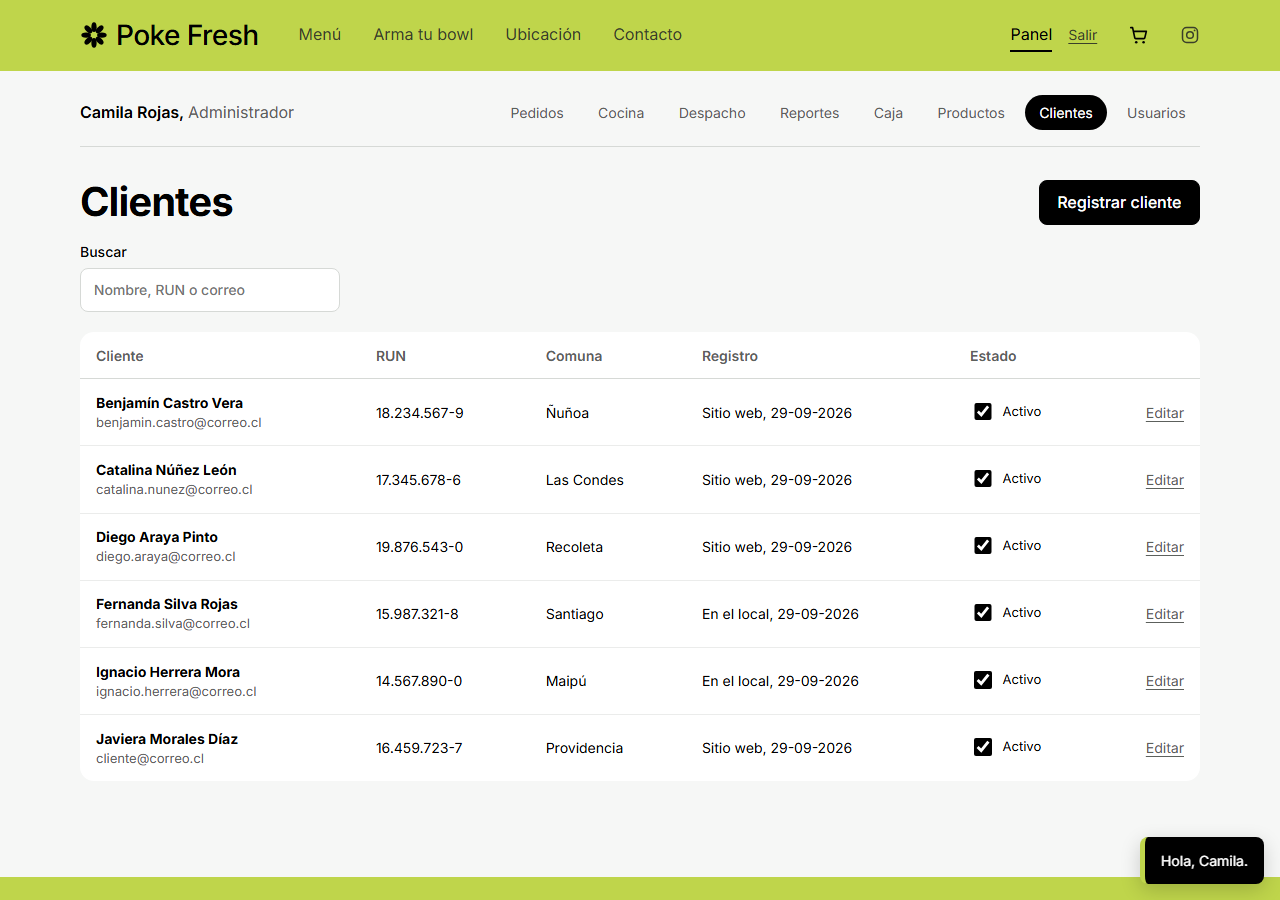
\includegraphics[width=\linewidth,height=0.42\textheight,keepaspectratio]{../evidencias/pantallas/13-clientes.png}
\captionof{figure}{Administración: clientes}
\end{minipage}
\end{figure}

\begin{figure}[H]\centering
\begin{minipage}[t]{0.485\linewidth}\centering
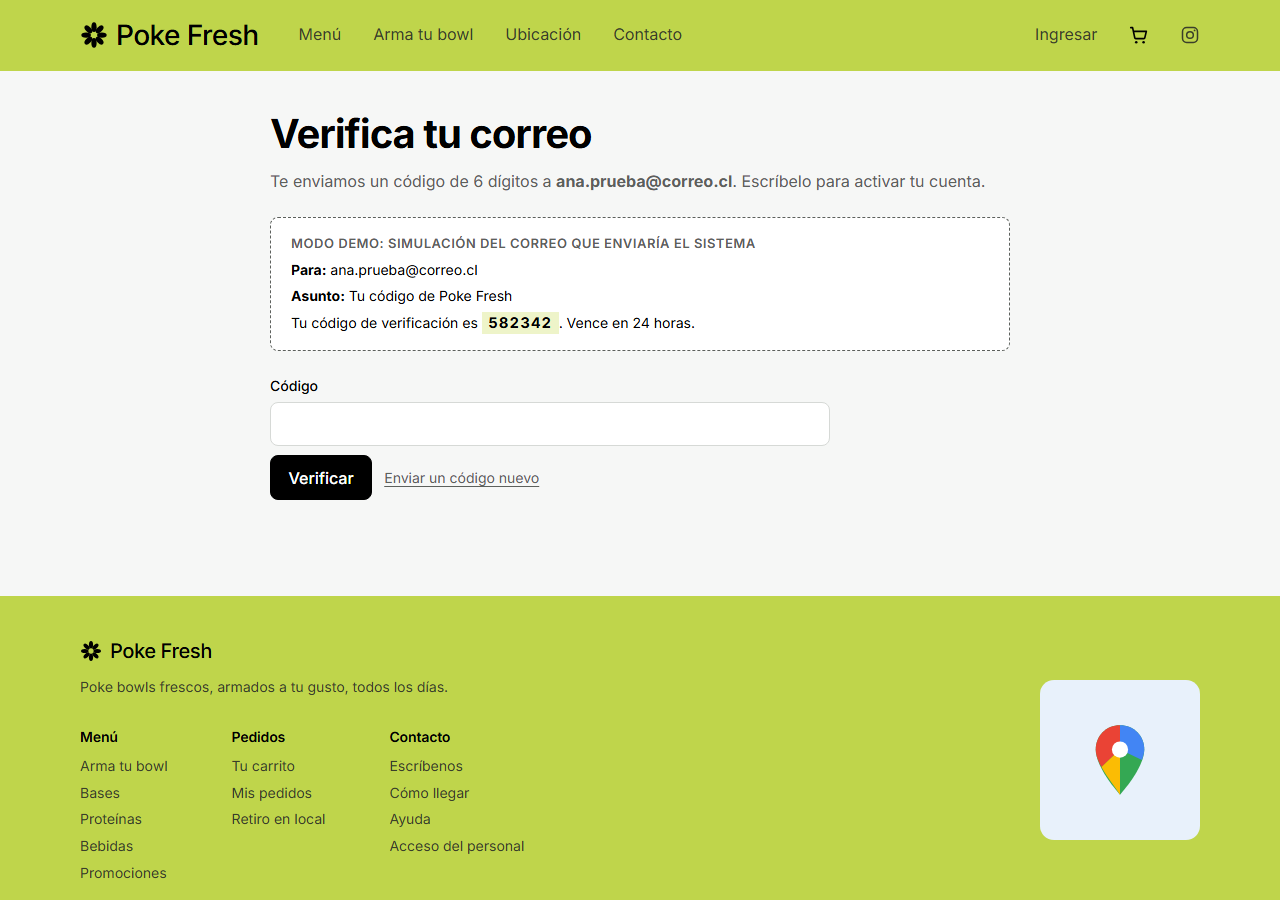
\includegraphics[width=\linewidth,height=0.42\textheight,keepaspectratio]{../evidencias/pantallas/15-verificacion-correo.png}
\captionof{figure}{Registro: verificación de correo (modo demo)}
\end{minipage}\hfill
\begin{minipage}[t]{0.485\linewidth}\centering
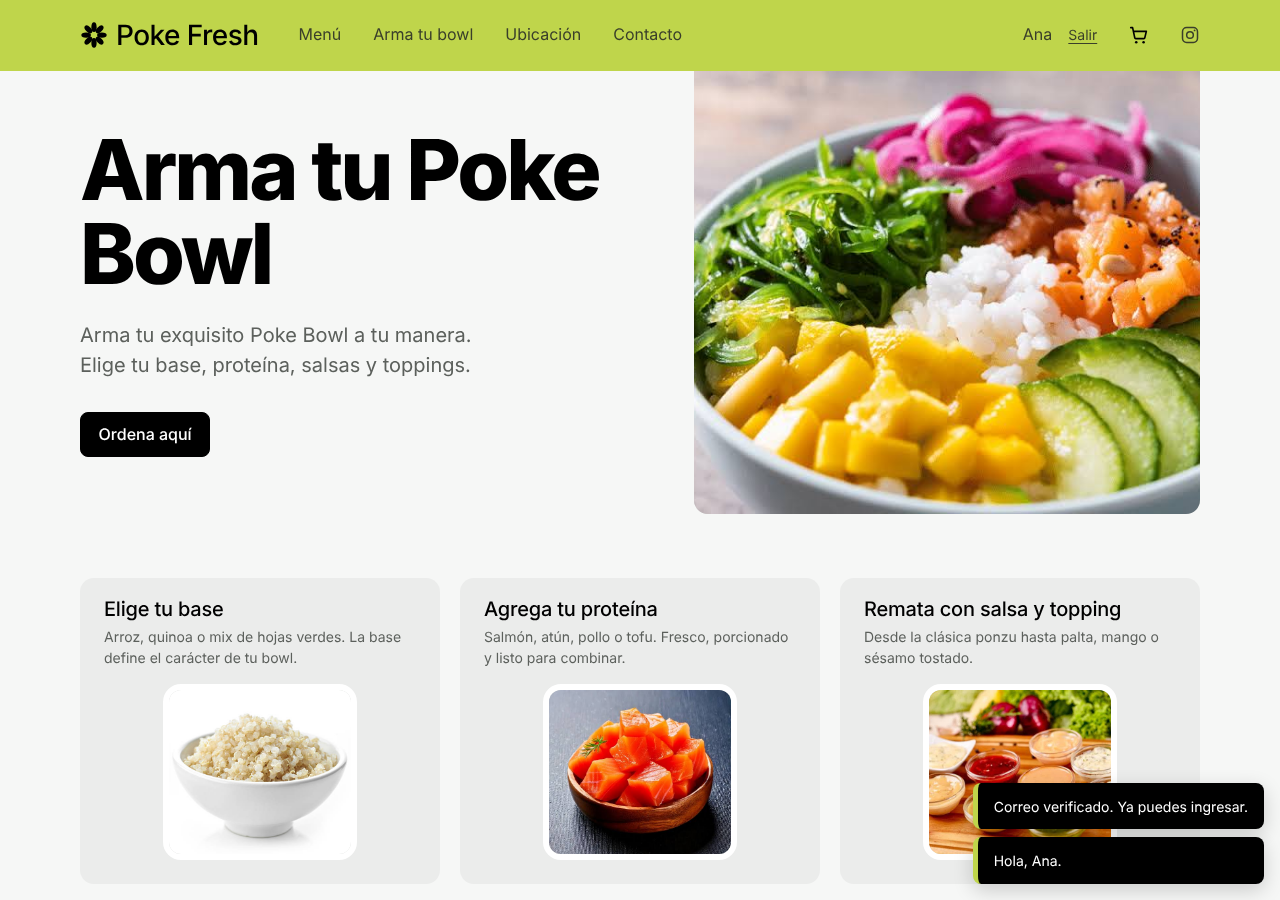
\includegraphics[width=\linewidth,height=0.42\textheight,keepaspectratio]{../evidencias/pantallas/16-cliente-nuevo-con-sesion.png}
\captionof{figure}{Cliente nuevo con sesión iniciada}
\end{minipage}
\end{figure}

\subsubsection{Teléfono emulado (Chromium, 390×812, táctil): compra completa}

\begin{figure}[H]\centering
\begin{minipage}[t]{0.242\linewidth}\centering
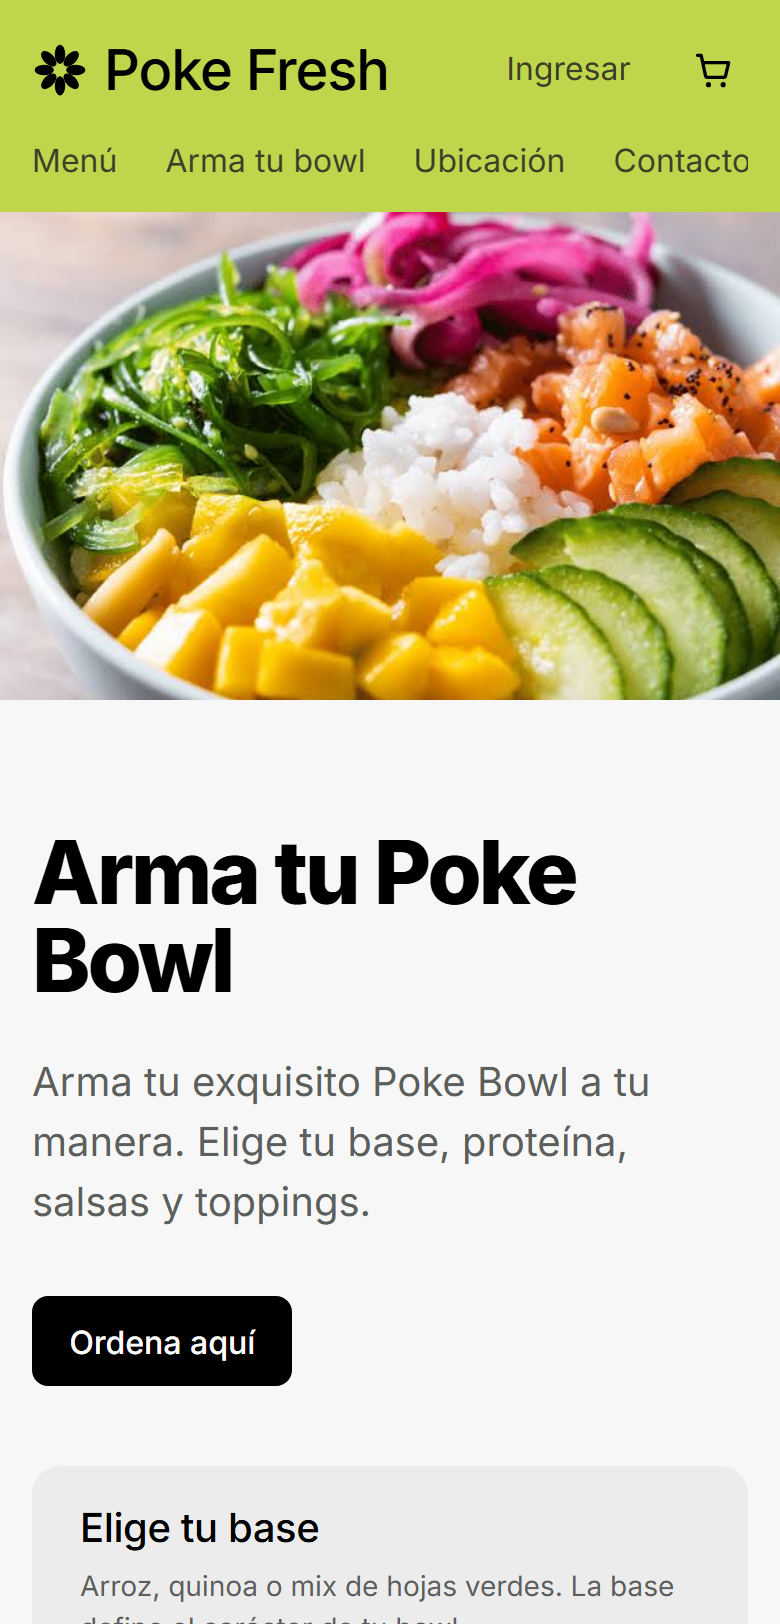
\includegraphics[width=\linewidth,height=0.4\textheight,keepaspectratio]{../evidencias/movil/01-inicio.png}
\captionof{figure}{Inicio}
\end{minipage}\hfill
\begin{minipage}[t]{0.242\linewidth}\centering
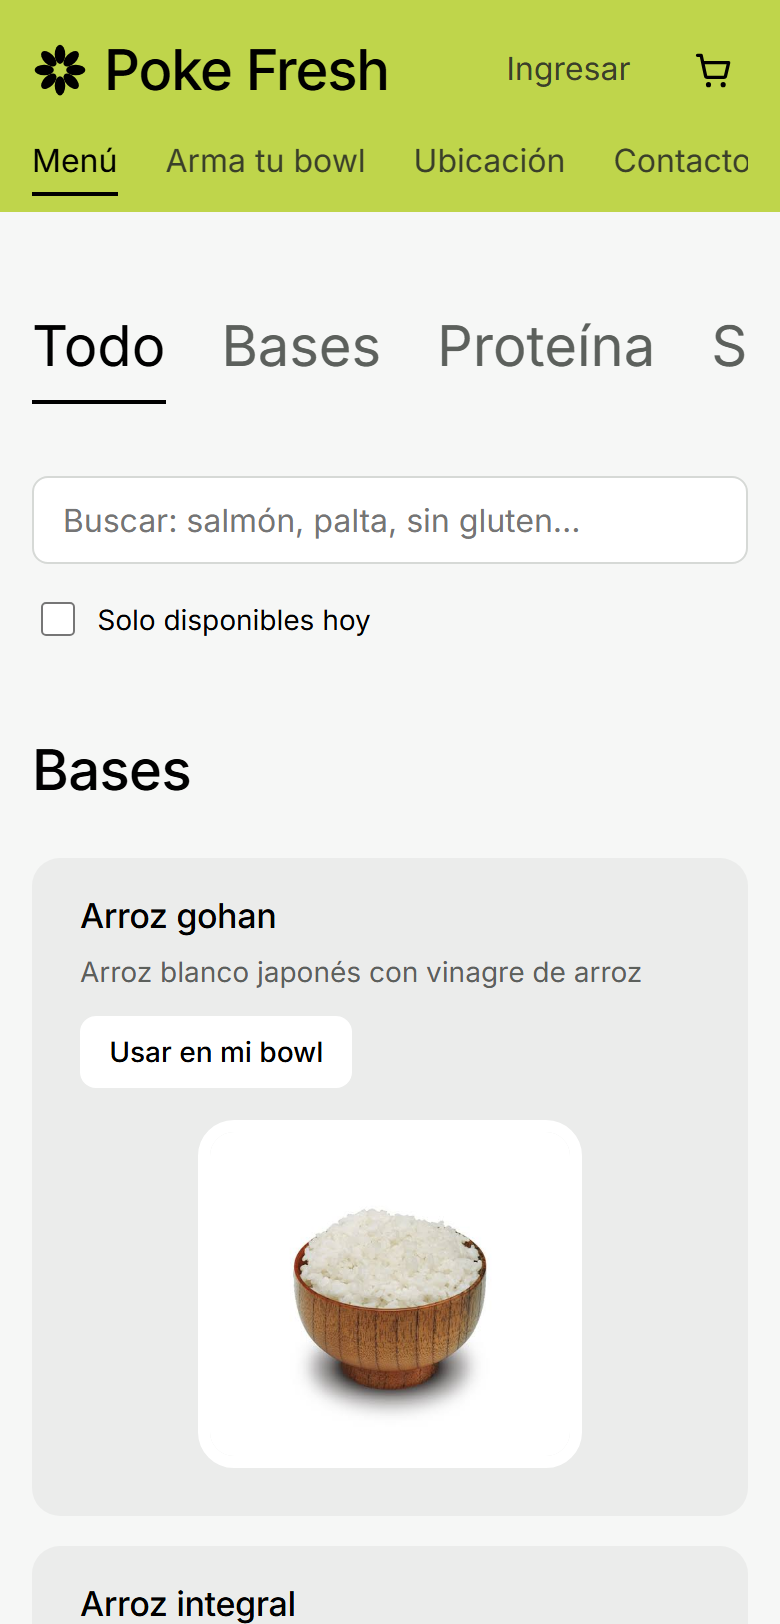
\includegraphics[width=\linewidth,height=0.4\textheight,keepaspectratio]{../evidencias/movil/02-menu.png}
\captionof{figure}{Menú}
\end{minipage}\hfill
\begin{minipage}[t]{0.242\linewidth}\centering
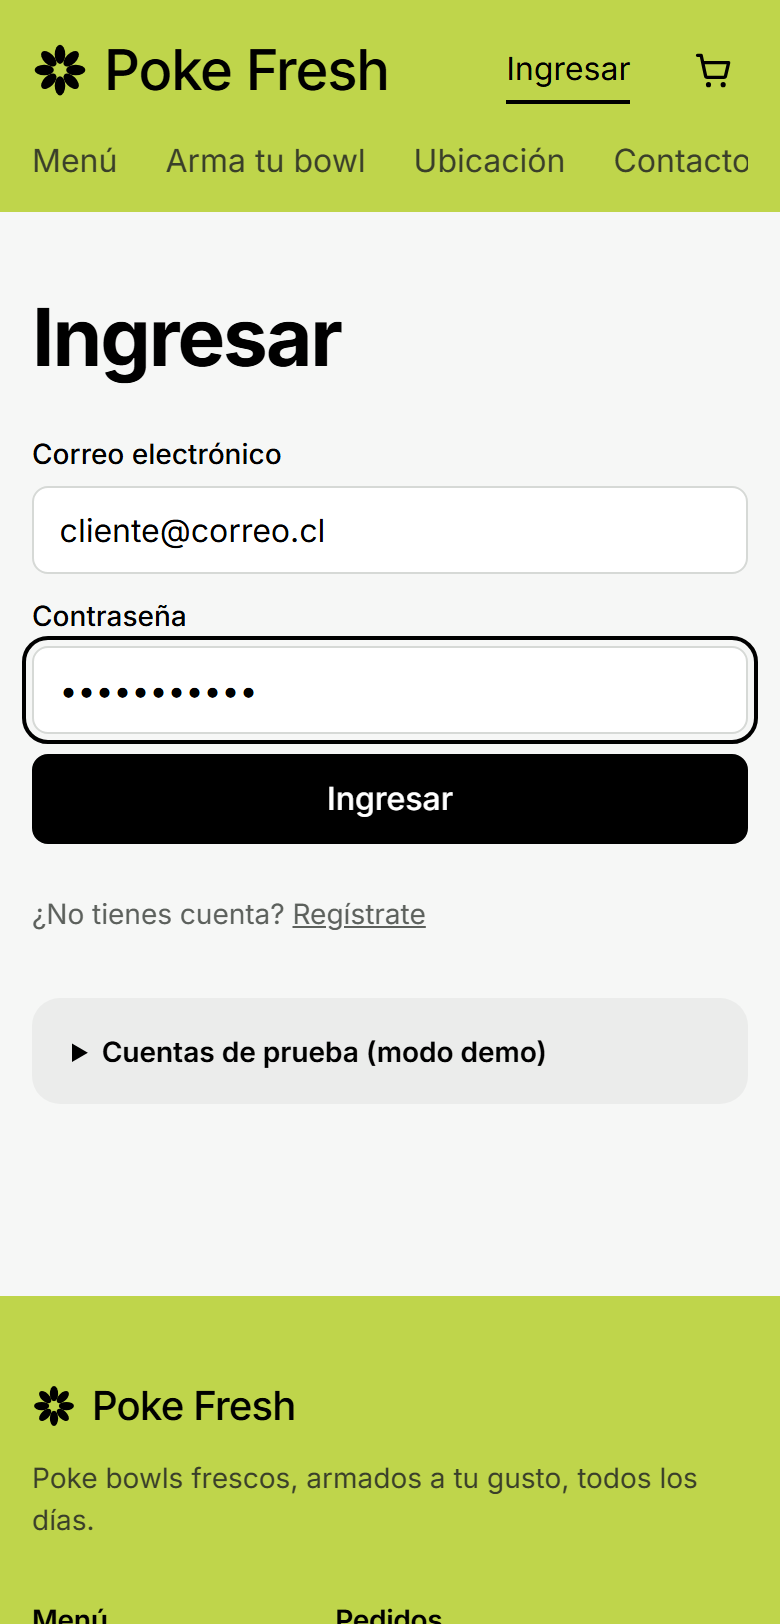
\includegraphics[width=\linewidth,height=0.4\textheight,keepaspectratio]{../evidencias/movil/03-ingreso.png}
\captionof{figure}{Ingreso}
\end{minipage}\hfill
\begin{minipage}[t]{0.242\linewidth}\centering
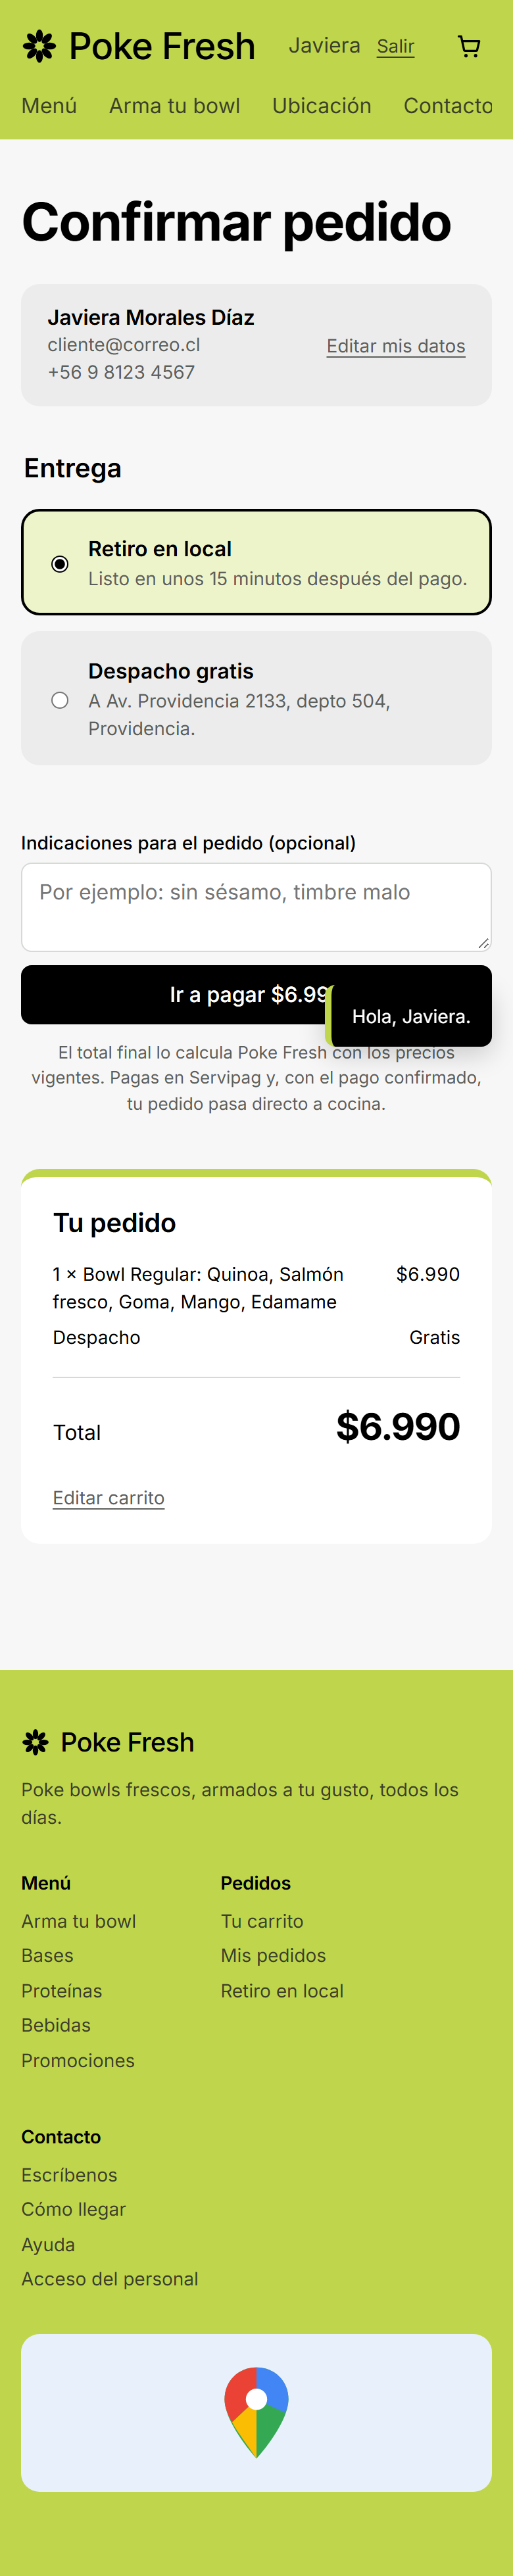
\includegraphics[width=\linewidth,height=0.4\textheight,keepaspectratio]{../evidencias/movil/04-checkout.png}
\captionof{figure}{Checkout}
\end{minipage}
\end{figure}

\begin{figure}[H]\centering
\begin{minipage}[t]{0.242\linewidth}\centering
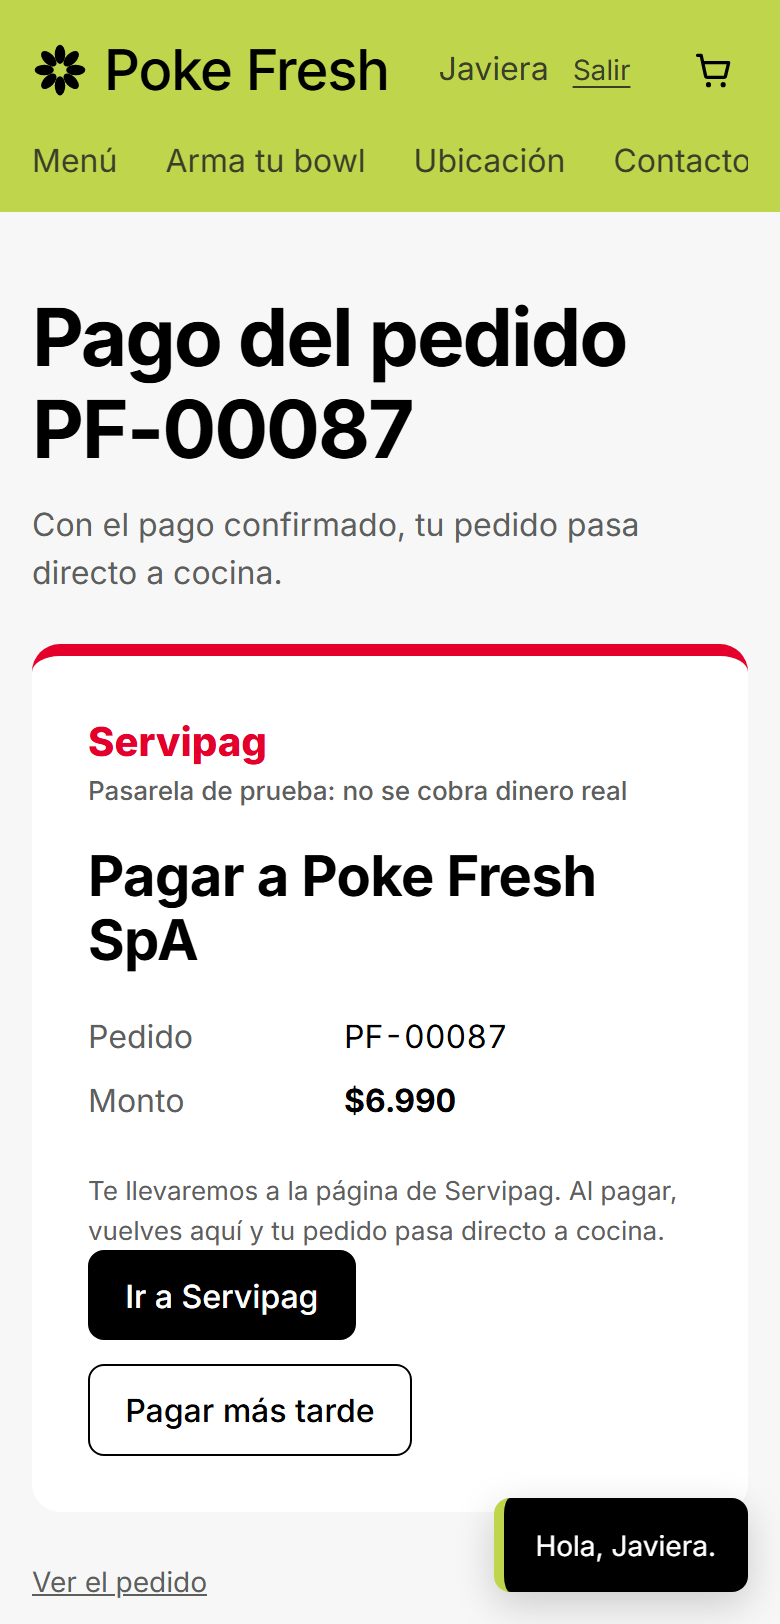
\includegraphics[width=\linewidth,height=0.4\textheight,keepaspectratio]{../evidencias/movil/05-pago.png}
\captionof{figure}{Pago}
\end{minipage}\hfill
\begin{minipage}[t]{0.242\linewidth}\centering
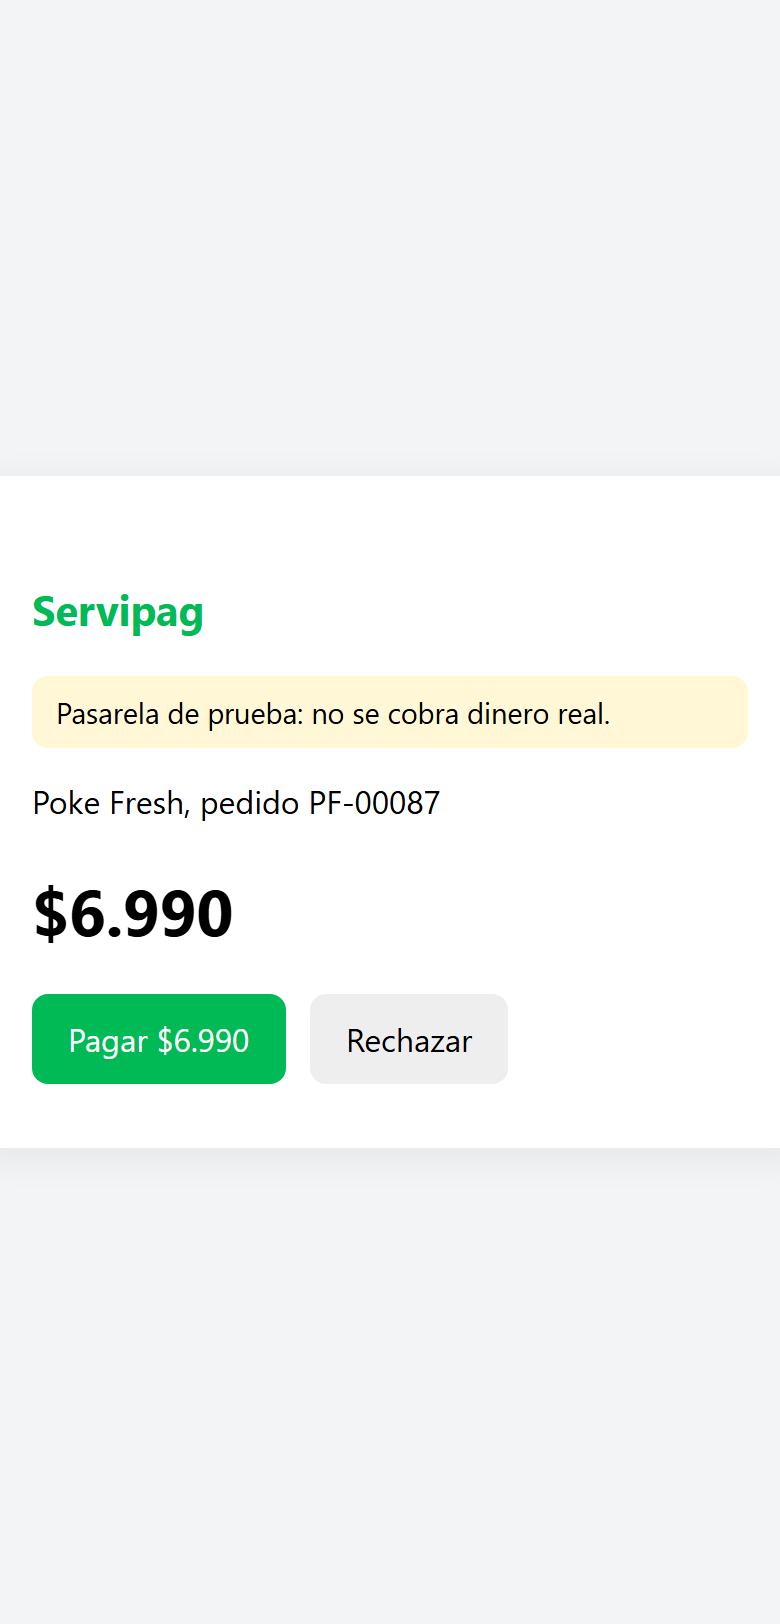
\includegraphics[width=\linewidth,height=0.4\textheight,keepaspectratio]{../evidencias/movil/06-pasarela-servipag.png}
\captionof{figure}{Pasarela Servipag}
\end{minipage}\hfill
\begin{minipage}[t]{0.242\linewidth}\centering
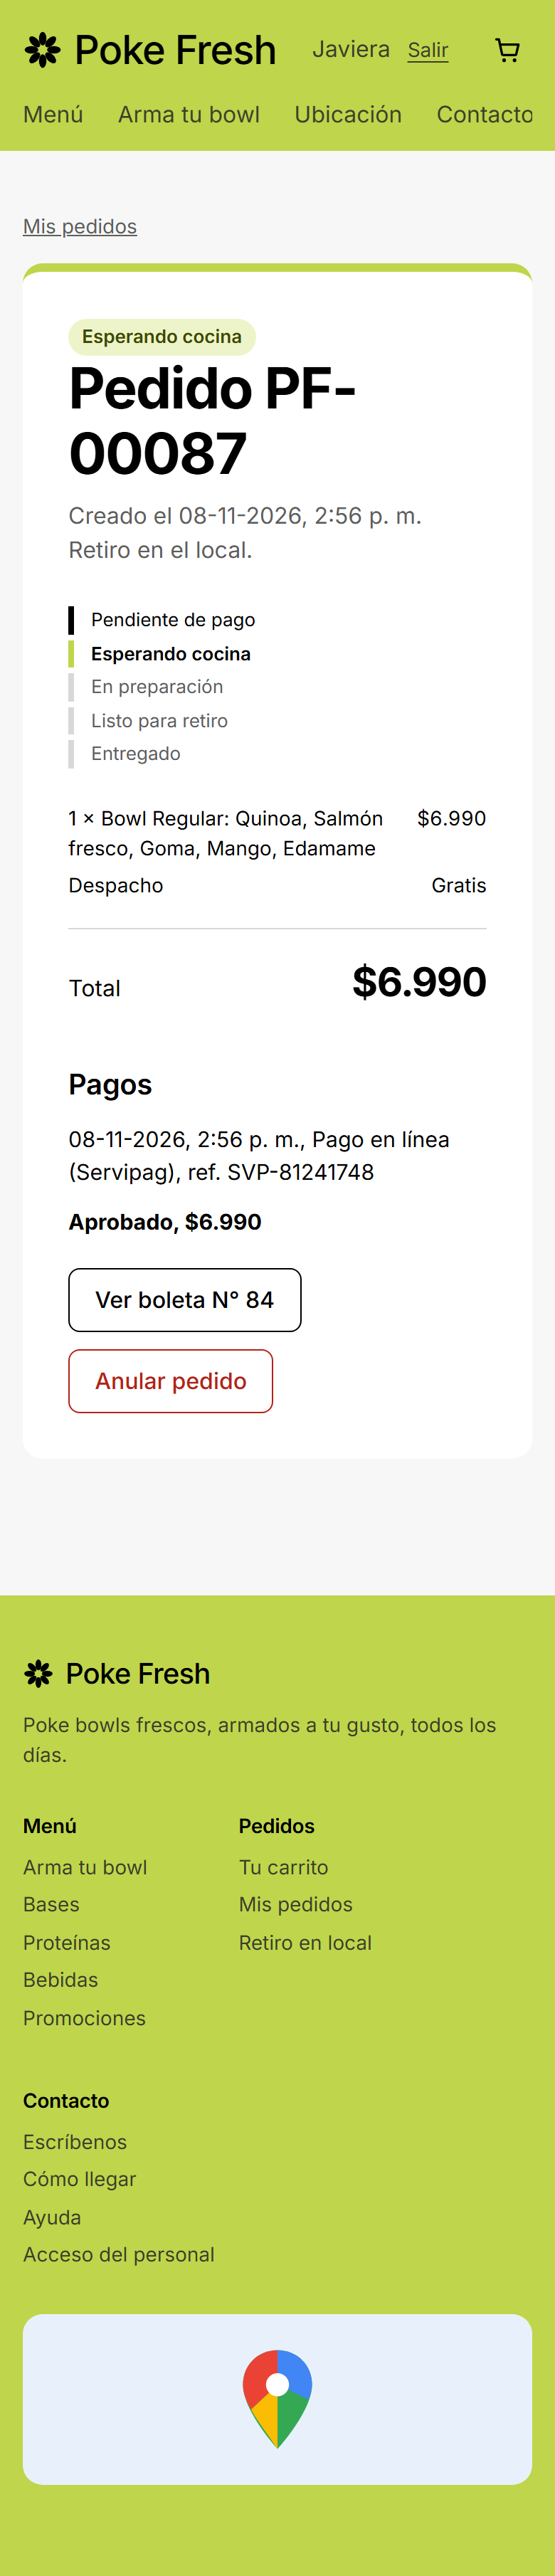
\includegraphics[width=\linewidth,height=0.4\textheight,keepaspectratio]{../evidencias/movil/07-pedido-pagado.png}
\captionof{figure}{Pedido pagado con boleta}
\end{minipage}\hfill
\begin{minipage}[t]{0.242\linewidth}\centering
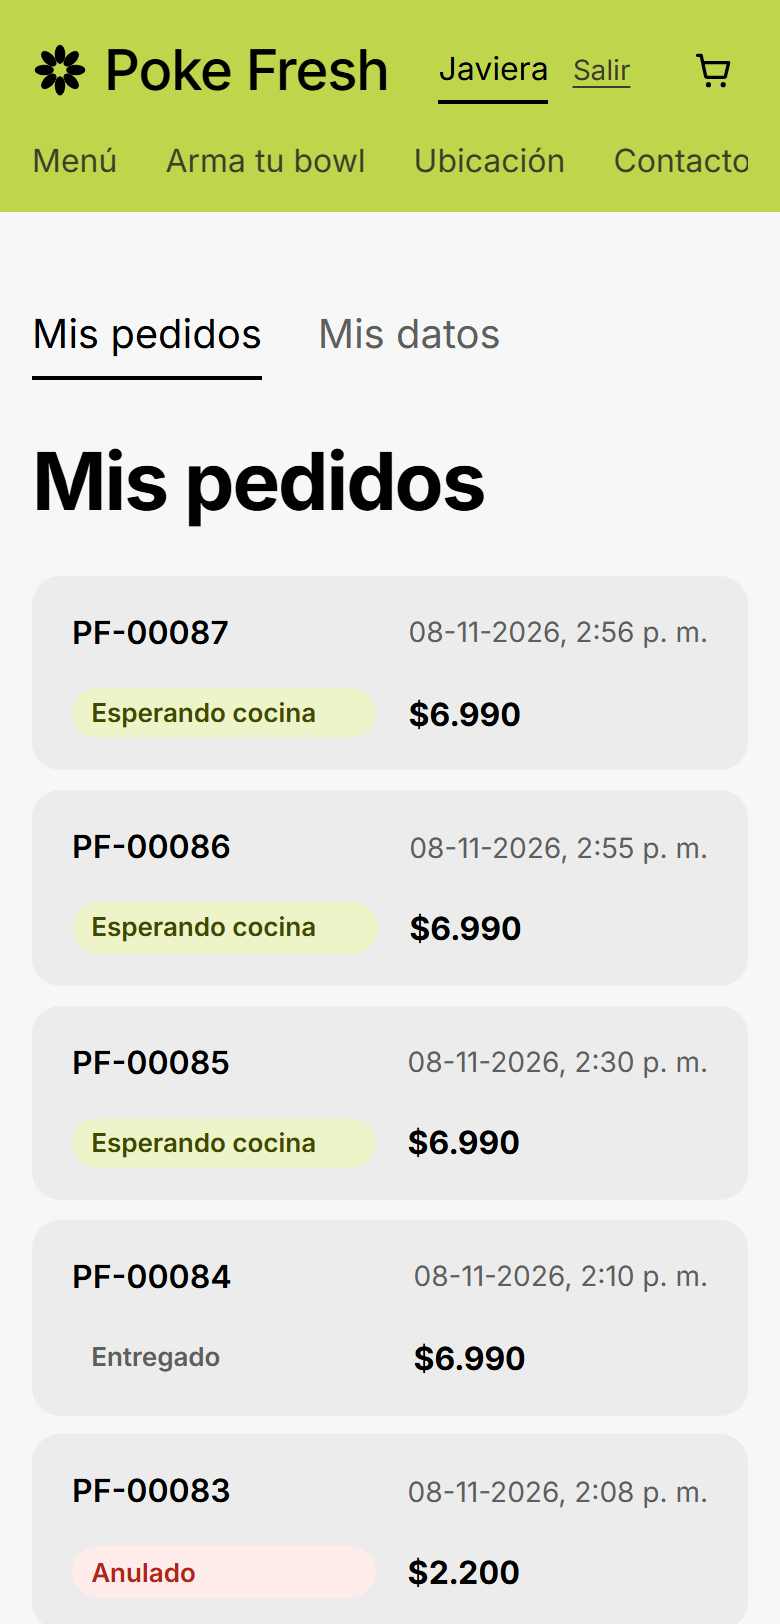
\includegraphics[width=\linewidth,height=0.4\textheight,keepaspectratio]{../evidencias/movil/08-mis-pedidos.png}
\captionof{figure}{Mis pedidos}
\end{minipage}
\end{figure}

Es una emulación en Chromium, no un teléfono real.


\subsubsection{Navegador real (Microsoft Edge): compra completa por HTTPS}

\begin{figure}[H]\centering
\begin{minipage}[t]{0.485\linewidth}\centering
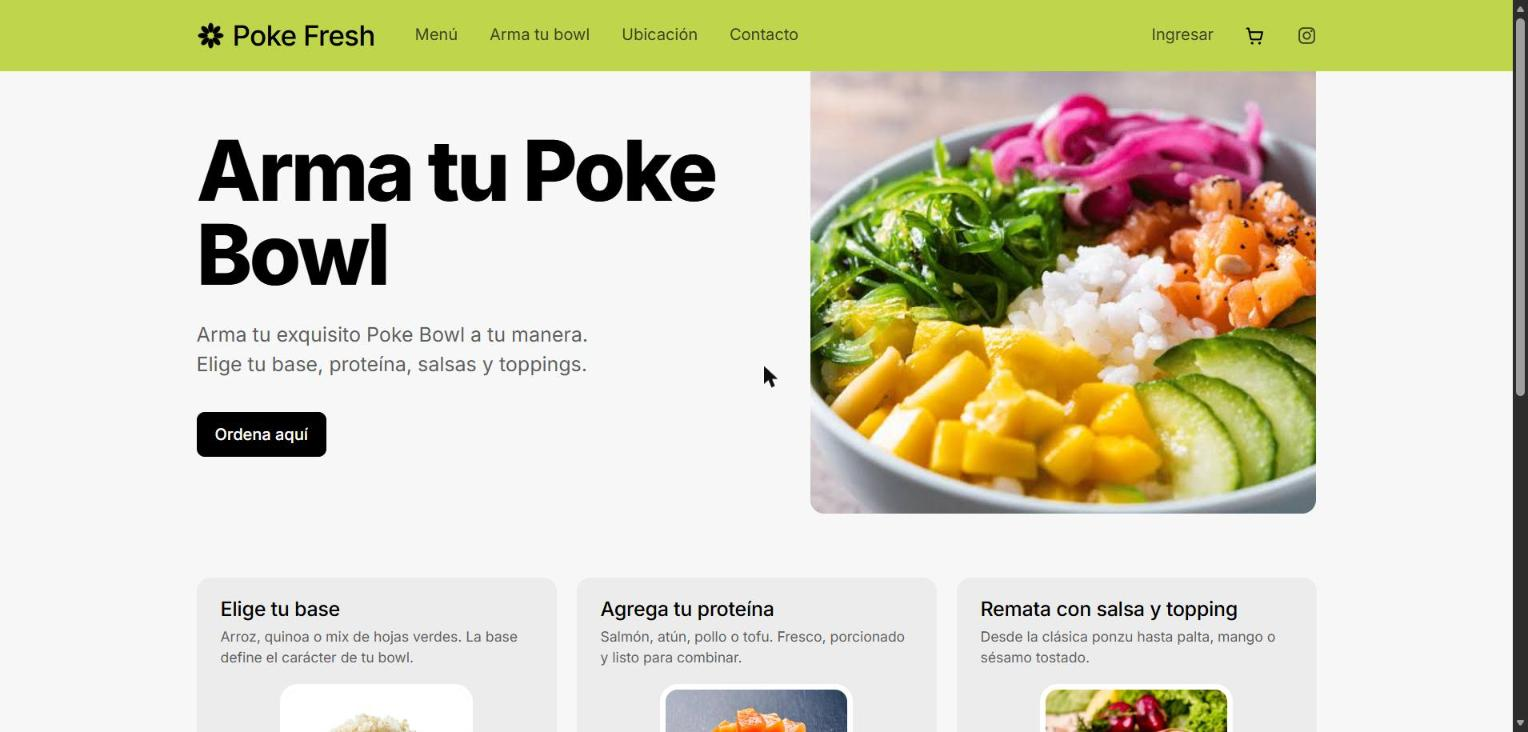
\includegraphics[width=\linewidth,height=0.42\textheight,keepaspectratio]{../evidencias/navegador-real/01-inicio.jpg}
\captionof{figure}{Inicio}
\end{minipage}\hfill
\begin{minipage}[t]{0.485\linewidth}\centering
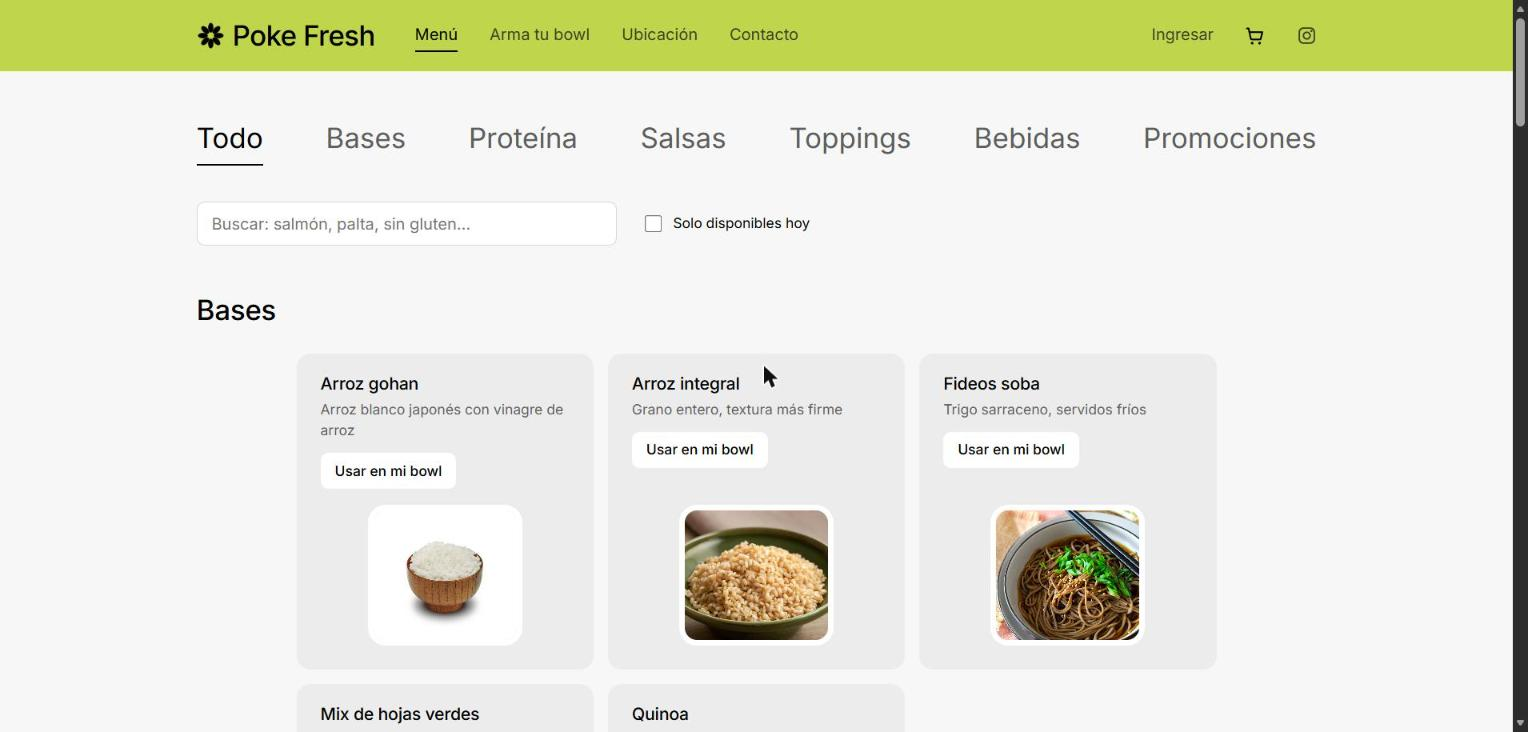
\includegraphics[width=\linewidth,height=0.42\textheight,keepaspectratio]{../evidencias/navegador-real/02-menu.jpg}
\captionof{figure}{Menú}
\end{minipage}
\end{figure}

\begin{figure}[H]\centering
\begin{minipage}[t]{0.485\linewidth}\centering
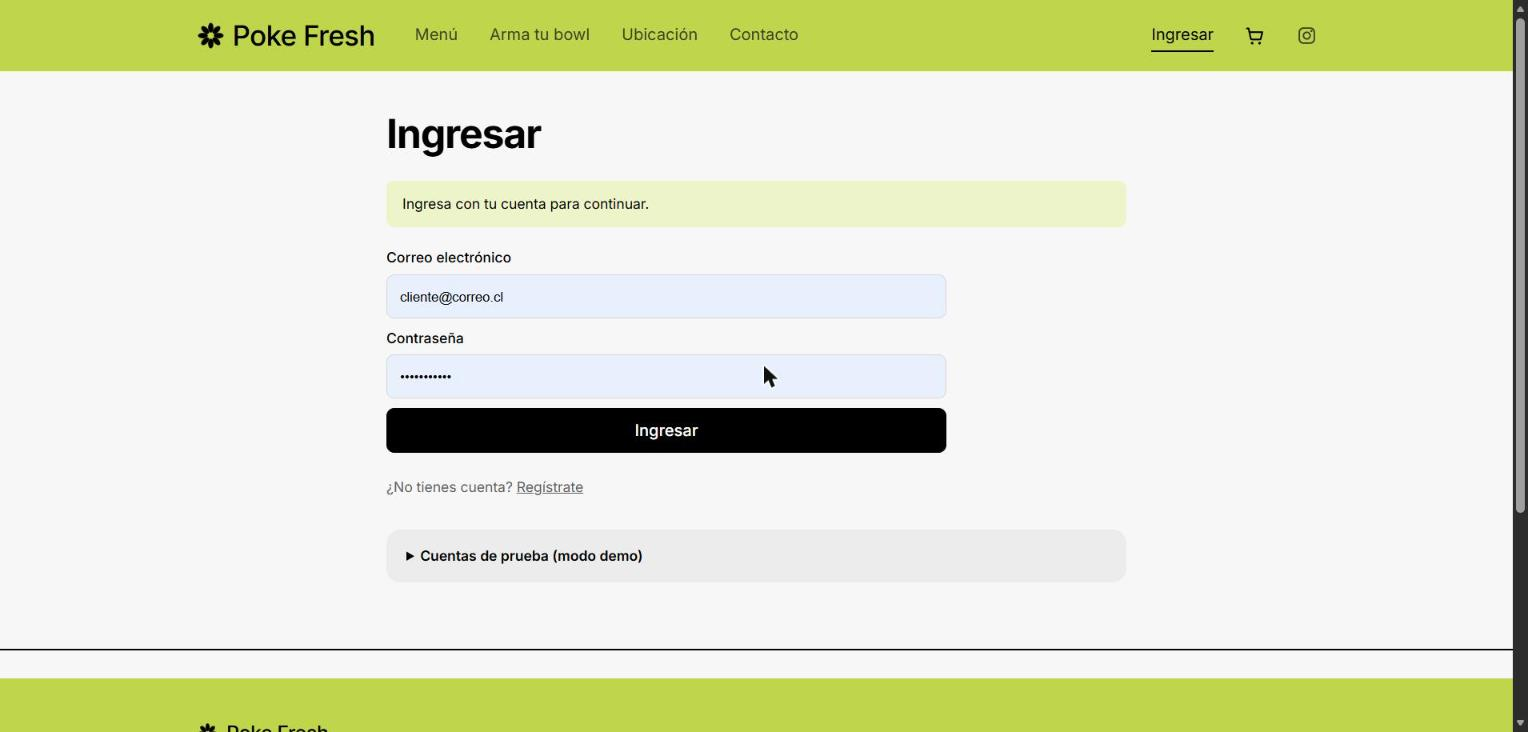
\includegraphics[width=\linewidth,height=0.42\textheight,keepaspectratio]{../evidencias/navegador-real/03-ingreso.jpg}
\captionof{figure}{Ingreso}
\end{minipage}\hfill
\begin{minipage}[t]{0.485\linewidth}\centering
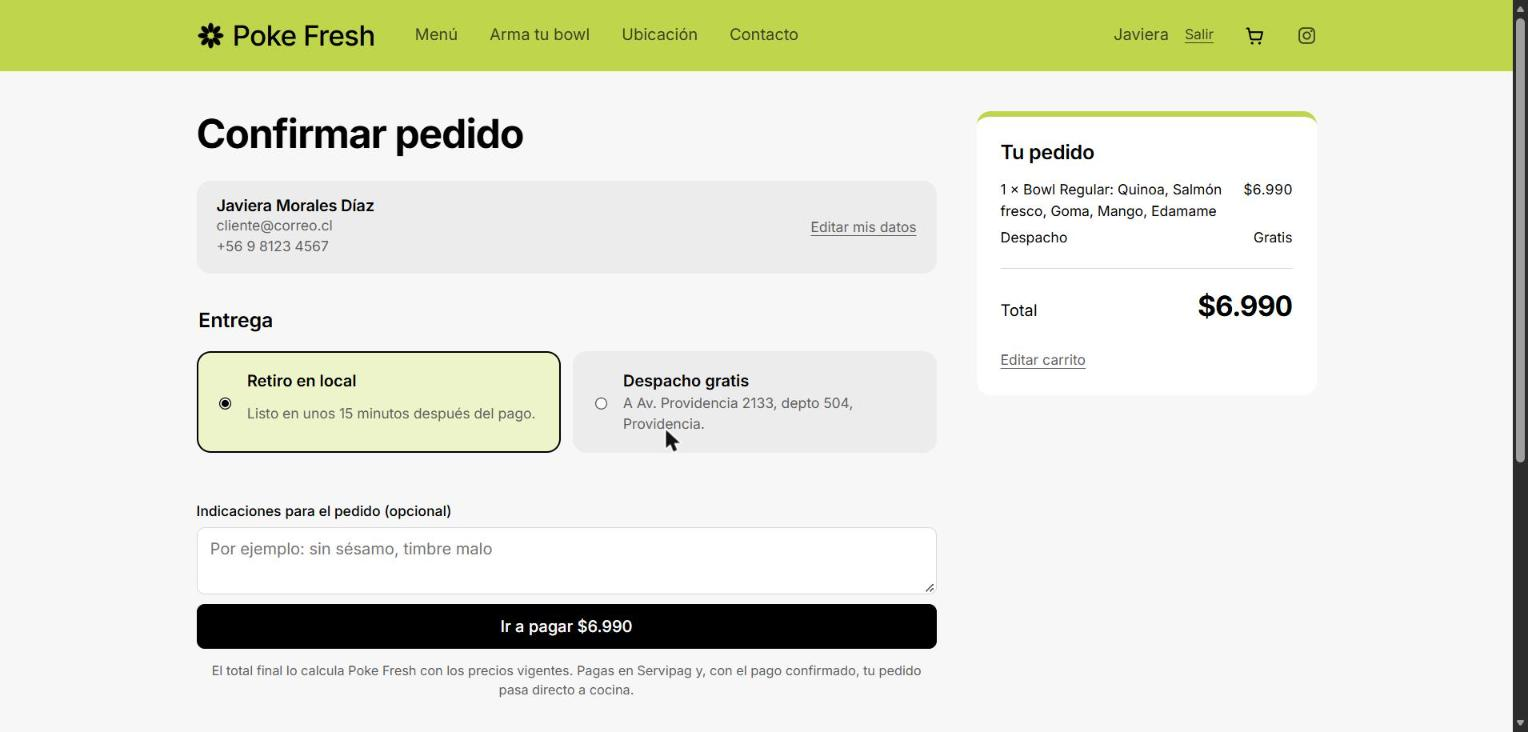
\includegraphics[width=\linewidth,height=0.42\textheight,keepaspectratio]{../evidencias/navegador-real/04-checkout.jpg}
\captionof{figure}{Checkout}
\end{minipage}
\end{figure}

\begin{figure}[H]\centering
\begin{minipage}[t]{0.485\linewidth}\centering
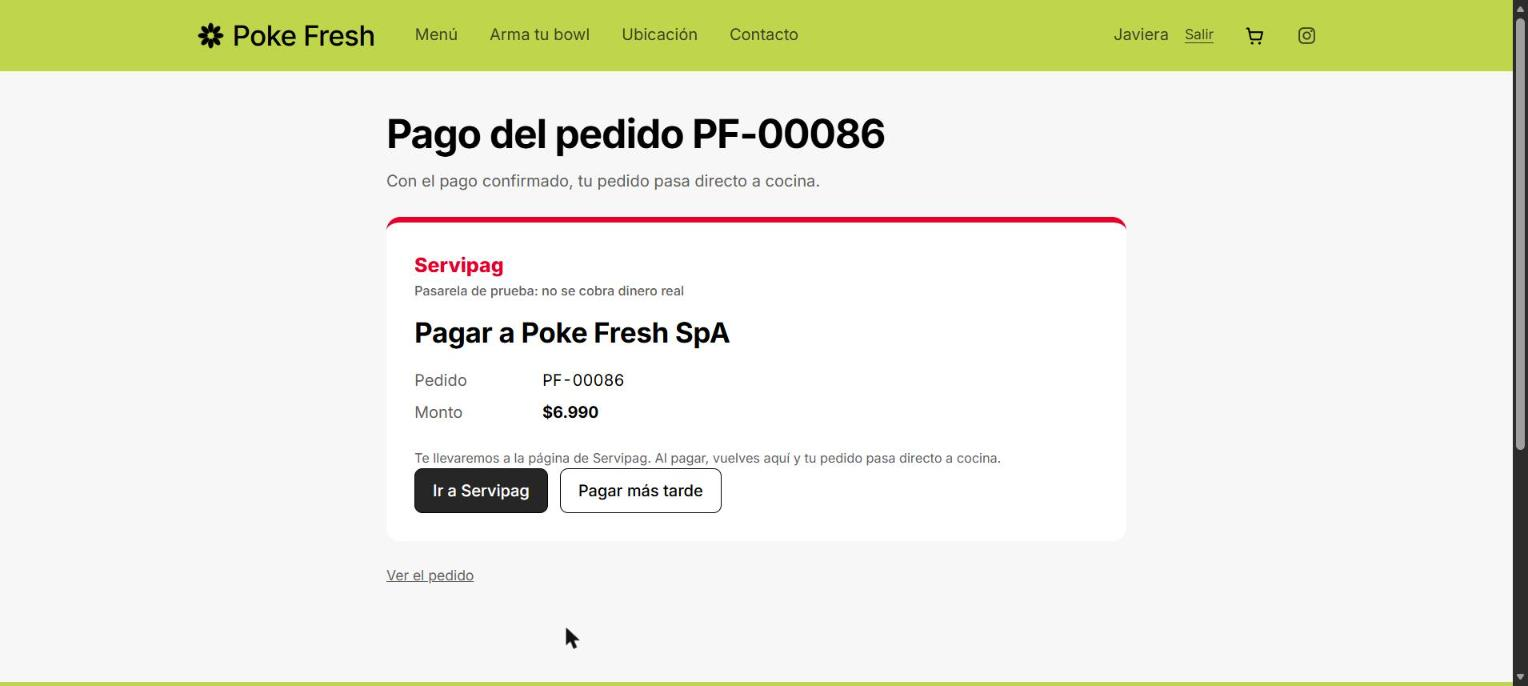
\includegraphics[width=\linewidth,height=0.42\textheight,keepaspectratio]{../evidencias/navegador-real/05-pago.jpg}
\captionof{figure}{Pago}
\end{minipage}\hfill
\begin{minipage}[t]{0.485\linewidth}\centering
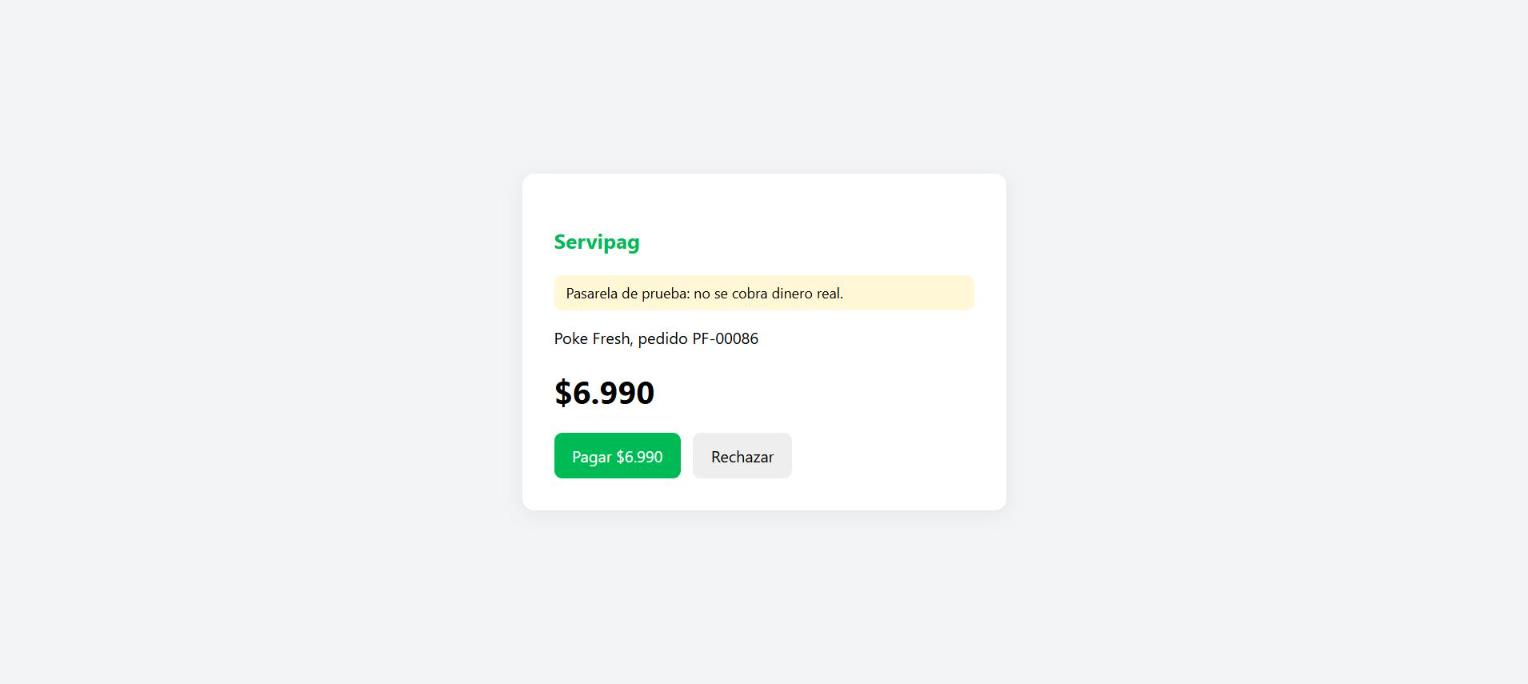
\includegraphics[width=\linewidth,height=0.42\textheight,keepaspectratio]{../evidencias/navegador-real/06-pasarela-servipag.jpg}
\captionof{figure}{Pasarela de pago en https://localhost:9000}
\end{minipage}
\end{figure}

\begin{figure}[H]\centering
\begin{minipage}[t]{0.485\linewidth}\centering
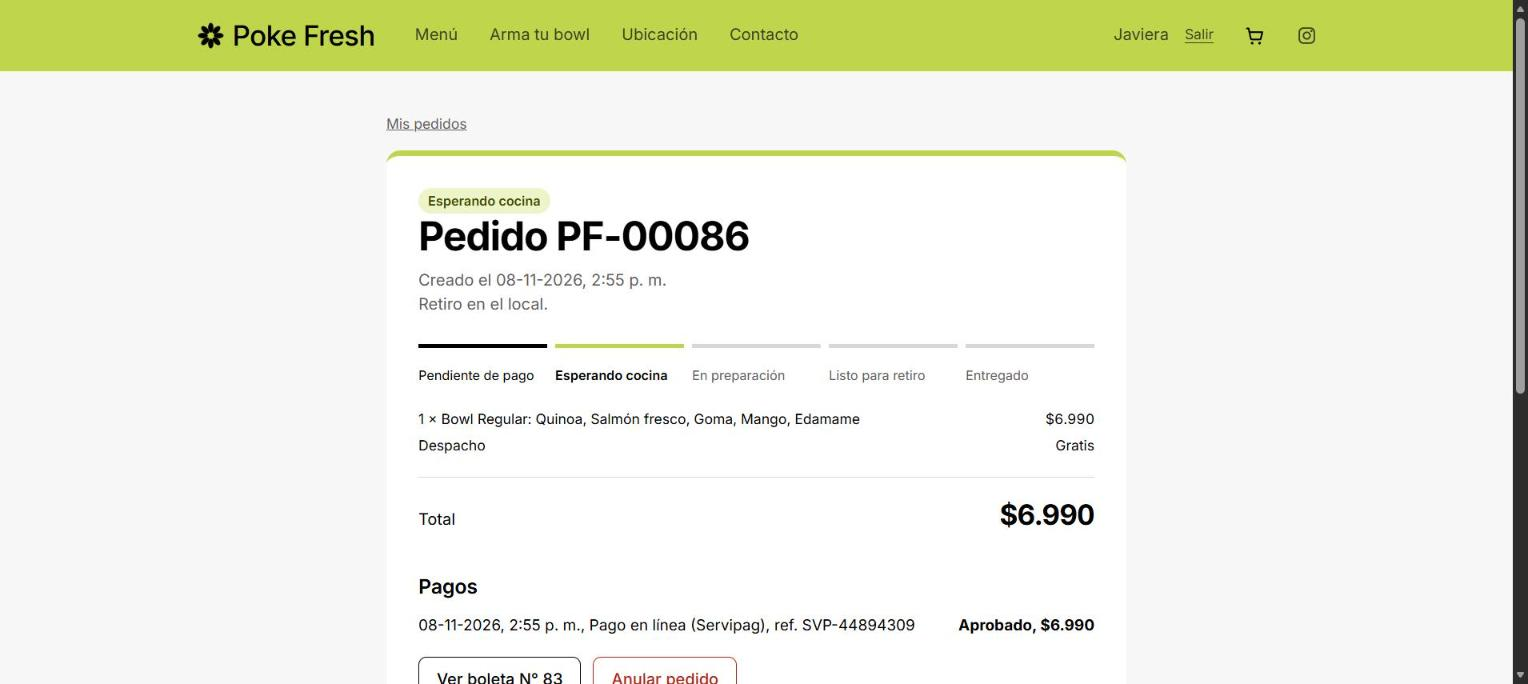
\includegraphics[width=\linewidth,height=0.42\textheight,keepaspectratio]{../evidencias/navegador-real/07-pedido-pagado.jpg}
\captionof{figure}{Pedido pagado}
\end{minipage}\hfill
\begin{minipage}[t]{0.485\linewidth}\centering
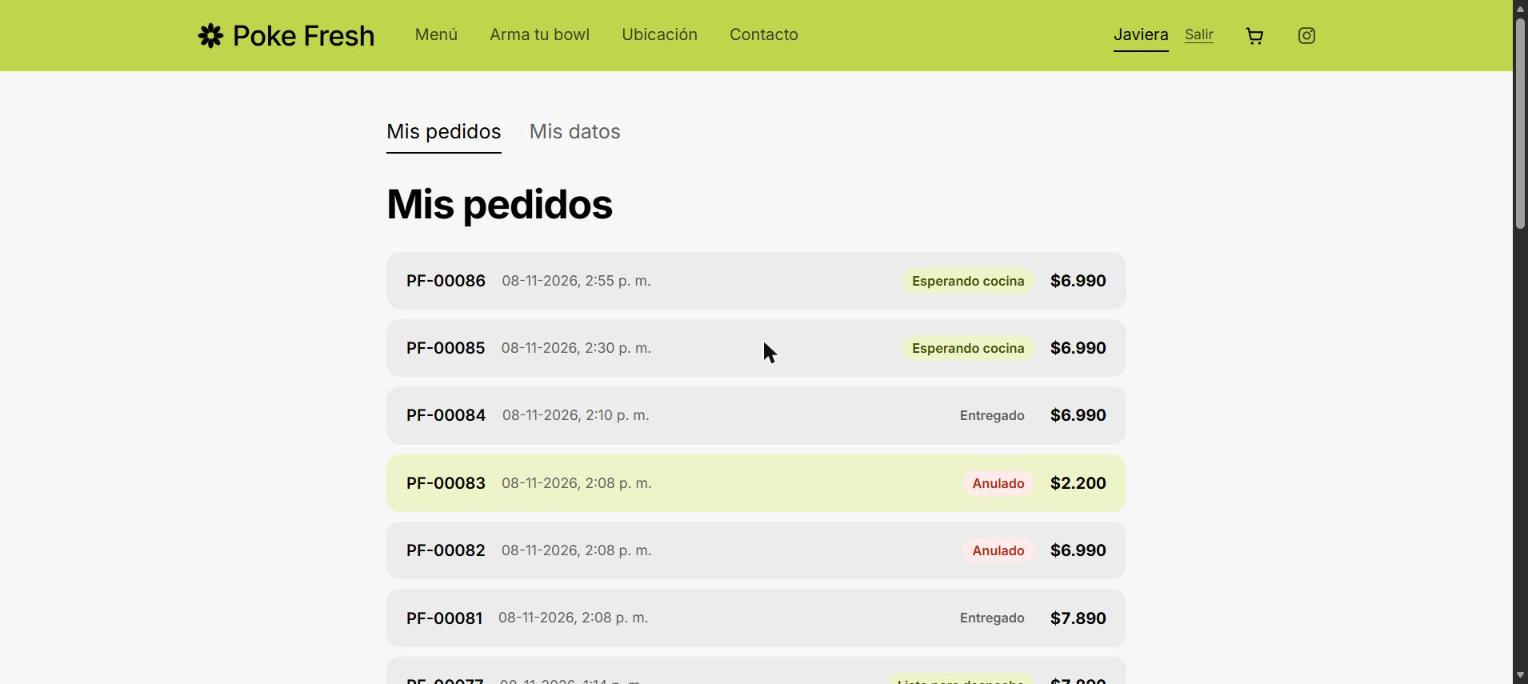
\includegraphics[width=\linewidth,height=0.42\textheight,keepaspectratio]{../evidencias/navegador-real/08-mis-pedidos.jpg}
\captionof{figure}{Mis pedidos}
\end{minipage}
\end{figure}

Las capturas muestran la página y no la barra de direcciones; el protocolo consta en \texttt{evidencias/\allowbreak{}navegador-\allowbreak{}real/\allowbreak{}datos-\allowbreak{}navegador.\allowbreak{}json}.


\subsection{Matriz requisito, pantalla, servicio, prueba y evidencia}

{\footnotesize
\setlength{\tabcolsep}{3pt}\renewcommand{\arraystretch}{1.15}
\begin{longtable}{|>{\raggedright\arraybackslash}p{\dimexpr 0.0611\linewidth-2\tabcolsep\relax}|>{\raggedright\arraybackslash}p{\dimexpr 0.1268\linewidth-2\tabcolsep\relax}|>{\raggedright\arraybackslash}p{\dimexpr 0.2599\linewidth-2\tabcolsep\relax}|>{\raggedright\arraybackslash}p{\dimexpr 0.2682\linewidth-2\tabcolsep\relax}|>{\raggedright\arraybackslash}p{\dimexpr 0.0988\linewidth-2\tabcolsep\relax}|>{\raggedright\arraybackslash}p{\dimexpr 0.1851\linewidth-2\tabcolsep\relax}|}
\hline
\textbf{Req.} & \textbf{Pantalla} & \textbf{Servicio} & \textbf{Prueba} & \textbf{Resultado} & \textbf{Evidencia} \\ \hline
\endfirsthead
\hline
\textbf{Req.} & \textbf{Pantalla} & \textbf{Servicio} & \textbf{Prueba} & \textbf{Resultado} & \textbf{Evidencia} \\ \hline
\endhead
R1 & Menú, Arma tu bowl & inventario (S01 a S03) & \texttt{test\_\allowbreak{}catalogo\_\allowbreak{}publico.\allowbreak{}.\allowbreak{}.\allowbreak{}}, \texttt{test\_\allowbreak{}cotizacion.\allowbreak{}.\allowbreak{}.\allowbreak{}}, caso 7.1 & OK & \texttt{pantallas/\allowbreak{}02-\allowbreak{}menu-\allowbreak{}desde-\allowbreak{}inventario.\allowbreak{}png} \\ \hline
R2 & Arma tu bowl & inventario (S03) & \texttt{test\_\allowbreak{}reglas\_\allowbreak{}de\_\allowbreak{}armado.\allowbreak{}.\allowbreak{}.\allowbreak{}}, caso 10.1 & OK & e2e 10.1 \\ \hline
R3 & Promo & inventario (S03) & \texttt{test\_\allowbreak{}crear\_\allowbreak{}pedido\_\allowbreak{}calcula\_\allowbreak{}total.\allowbreak{}.\allowbreak{}.\allowbreak{}} (cotizador de promos en \texttt{reglas.\allowbreak{}py}) & OK & — \\ \hline
R4 & Carrito & frontend + inventario (S03, S15) & recorrido de pantallas & OK & \texttt{pantallas/\allowbreak{}03-\allowbreak{}checkout.\allowbreak{}png} \\ \hline
R5 & Registro, Verificar & clientes + Auth (S07, S38, S39) & \texttt{test\_\allowbreak{}registro\_\allowbreak{}crea\_\allowbreak{}ficha.\allowbreak{}.\allowbreak{}.\allowbreak{}}, \texttt{cuenta nueva de cliente.\allowbreak{}.\allowbreak{}.\allowbreak{}} & OK & \texttt{pantallas/\allowbreak{}15-\allowbreak{}verificacion-\allowbreak{}correo.\allowbreak{}png}, \texttt{16-\allowbreak{}.\allowbreak{}.\allowbreak{}.\allowbreak{}} \\ \hline
R6 & Ingresar, Panel & Auth + gateway (S33 a S36, S40 a S43) & casos 7.3, 7.8, 7.11 & OK & e2e \\ \hline
R7 & Confirmar pedido & pedidos + clientes (S15) & \texttt{test\_\allowbreak{}despacho\_\allowbreak{}fuera\_\allowbreak{}de\_\allowbreak{}radio}, caso 10.1 & OK & e2e 10.1 \\ \hline
R8 & Pago, Pedido, Boleta & pagos + pasarela + pedidos + ActiveMQ (S27, S29, S18) & \texttt{test\_\allowbreak{}pago\_\allowbreak{}completo\_\allowbreak{}por\_\allowbreak{}la\_\allowbreak{}pasarela}, casos 7.6, 10.2, 10.3 & OK & \texttt{pantallas/\allowbreak{}04} a \texttt{06}; log del notificador \\ \hline
R9 & Cocina & pedidos (S16, S20, S21, S24) & \texttt{test\_\allowbreak{}flujo\_\allowbreak{}de\_\allowbreak{}cocina\_\allowbreak{}y\_\allowbreak{}despacho.\allowbreak{}.\allowbreak{}.\allowbreak{}}, caso 10.4 & OK & \texttt{pantallas/\allowbreak{}07-\allowbreak{}cocina.\allowbreak{}png} \\ \hline
R10 & Despacho & pedidos (S22, S23) & caso 10.4 & OK & \texttt{pantallas/\allowbreak{}08-\allowbreak{}despacho.\allowbreak{}png}, \texttt{09-\allowbreak{}.\allowbreak{}.\allowbreak{}.\allowbreak{}} \\ \hline
R11 & Pedido, Panel pedidos & pedidos + pagos + inventario (S25) & \texttt{test\_\allowbreak{}anular\_\allowbreak{}pedido\_\allowbreak{}pagado.\allowbreak{}.\allowbreak{}.\allowbreak{}}, \texttt{test\_\allowbreak{}no\_\allowbreak{}se\_\allowbreak{}anula.\allowbreak{}.\allowbreak{}.\allowbreak{}}, casos 10.5, 10.6 & OK & e2e \\ \hline
R12 & Productos, Clientes, Usuarios & inventario, clientes, Auth (S04 a S06, S10 a S14, S40 a S43) & \texttt{test\_\allowbreak{}solo\_\allowbreak{}admin\_\allowbreak{}elimina.\allowbreak{}.\allowbreak{}.\allowbreak{}}, \texttt{test\_\allowbreak{}admin\_\allowbreak{}registra\_\allowbreak{}en\_\allowbreak{}local.\allowbreak{}.\allowbreak{}.\allowbreak{}}, \texttt{solo un admin gestiona usuarios.\allowbreak{}.\allowbreak{}.\allowbreak{}} & OK & \texttt{pantallas/\allowbreak{}12}, \texttt{13} \\ \hline
R13 & Caja, Reportes & pedidos + GraphQL (S26, S32) & \texttt{test\_\allowbreak{}reporte\_\allowbreak{}de\_\allowbreak{}ventas.\allowbreak{}.\allowbreak{}.\allowbreak{}}, caso 8.3 & OK & \texttt{pantallas/\allowbreak{}11-\allowbreak{}reportes-\allowbreak{}graphql.\allowbreak{}png} \\ \hline
R14 & Pedido, Mis pedidos, Boleta & pedidos + GraphQL (S08, S09, S16 a S18, S30) & caso 7.5, 8.1 & OK & \texttt{pantallas/\allowbreak{}09}, \texttt{10} \\ \hline
\end{longtable}
}

\subsection{Ejemplo de autorización por pedido}

Con la misma regla (“un cliente solo ve sus pedidos”, aplicada por el servicio de pedidos):


\begin{itemize}[nosep,leftmargin=*]
\item \textbf{Autorizada:} la cliente \texttt{cli\_\allowbreak{}demo\_\allowbreak{}1} pide \texttt{GET /\allowbreak{}api/\allowbreak{}v1/\allowbreak{}pedidos/\allowbreak{}PF-\allowbreak{}00081} $\rightarrow$ \texttt{200} con su pedido.
\item \textbf{Denegada:} el cliente \texttt{cli\_\allowbreak{}demo\_\allowbreak{}2} pide lo mismo $\rightarrow$ \texttt{404 NO\_\allowbreak{}ENCONTRADO}, sin datos del pedido (no confirma ni que existe). Por GraphQL, \texttt{resumenPedido} responde \texttt{null}.
\end{itemize}

Ambas en el caso 7.5 (\texttt{evidencias/\allowbreak{}e2e-\allowbreak{}resultados.\allowbreak{}json}, con sus \texttt{X-\allowbreak{}Request-\allowbreak{}Id}, que se pueden buscar en \texttt{docker compose logs pedidos}).


\subsection{Operación}

\begin{itemize}[nosep,leftmargin=*]
\item \textbf{Iniciar y detener:} ver \texttt{README.\allowbreak{}md} (\texttt{docker compose up -\allowbreak{}d -\allowbreak{}-\allowbreak{}build}, \texttt{docker compose down}).
\item \textbf{Acceso:} \texttt{https:\allowbreak{}/\allowbreak{}/\allowbreak{}localhost:\allowbreak{}8080} (tienda y API) y \texttt{https:\allowbreak{}/\allowbreak{}/\allowbreak{}localhost:\allowbreak{}9000} (pasarela). Los certificados los firma una CA de prueba que crea \texttt{tls-\allowbreak{}init}, así que el navegador, o un antivirus que revise HTTPS, mostrará una advertencia en cada puerto; hay que aceptarla en ambos. Si otro programa ocupa el puerto 8080 en IPv4, hay que detenerlo (ver README).
\item \textbf{Configurar secretos:} solo \texttt{.\allowbreak{}env} con la clave raíz de Mongo; el resto lo crea \texttt{vault-\allowbreak{}init}. Para rotar un secreto: borrarlo en Vault y volver a correr \texttt{docker compose up -\allowbreak{}d} (excepto el pepper).
\item \textbf{Datos de prueba:} automáticos con \texttt{MODO\_\allowbreak{}DEMO=\allowbreak{}true} (servicio \texttt{semilla}).
\item \textbf{Health checks:} cada servicio tiene \texttt{/\allowbreak{}salud} (estado de Mongo y Vault), usado por Docker; \texttt{GET /\allowbreak{}api/\allowbreak{}salud} reúne todos.
\item \textbf{Logs:} una línea por petición con método, ruta, estado, duración, rol y \texttt{X-\allowbreak{}Request-\allowbreak{}Id}; sin cuerpos, correos ni tokens.
\item \textbf{Dependencias versionadas:} \texttt{package-\allowbreak{}lock.\allowbreak{}json} en cada proyecto Node, versiones fijas en \texttt{servicios/\allowbreak{}requirements.\allowbreak{}txt}, imágenes con versión (\texttt{mongo:\allowbreak{}7.\allowbreak{}0}, \texttt{hashicorp/\allowbreak{}vault:\allowbreak{}1.\allowbreak{}18}, \texttt{apache/\allowbreak{}activemq-\allowbreak{}classic:\allowbreak{}6.\allowbreak{}1.\allowbreak{}4}).
\end{itemize}
